%--------------------------------------------------------------------

\documentclass[
% -- opções da classe memoir --
12pt,				% tamanho da fonte
openright,			% capítulos começam em pág ímpar (insere página vazia)
twoside,			% para impressão em verso e anverso. Oposto a oneside
a4paper,			% tamanho do papel. 
oldfontcommands,
% -- opções da classe abntex2 --
chapter=TITLE,		% títulos de capítulos convertidos em letras maiúsculas
section=TITLE,		% títulos de seções convertidos em letras maiúsculas
%subsection=TITLE,	% títulos de subseções convertidos em letras maiúsculas
%subsubsection=TITLE,% títulos de subsubseções convertidos em letras maiúsculas
% -- opções do pacote babel --
french,				% idioma adicional para hifenização
spanish,			% idioma adicional para hifenização
brazil, 
english				% o último idioma é o principal do documento
]{abntex2}

% \setlength {\marginparwidth }{2cm}
% \usepackage{todonotes}
% ---
% Pacotes básicos 
% ---
%\usepackage{lmodern}% Usa a fonte Latin Modern	
\usepackage{rotating}
\usepackage{times}
\usepackage[T1]{fontenc}		% Selecao de codigos de fonte.
\usepackage[utf8]{inputenc}		% Codificacao do documento (conversão automática dos acentos)
\usepackage{lastpage}			% Usado pela Ficha catalográfica
\usepackage{indentfirst}		% Indenta o primeiro parágrafo de cada seção.
\usepackage{color}				% Controle das cores
\usepackage{graphicx}			% Inclusão de gráficos
\usepackage{microtype} 			% para melhorias de justificação
\usepackage{float}
\usepackage{subcaption}
\usepackage{multirow}
\usepackage{bigstrut}
\usepackage{booktabs}
\usepackage{listings}
\usepackage{xcolor}
\usepackage{comment}
\usepackage{pdflscape}
\usepackage{verbatimbox}
\usepackage{makecell}
\usepackage{pbox}
\usepackage{comment}
\usepackage{bm}

\usepackage{hyperref}
\hypersetup{
    colorlinks=true,
    linkcolor=blue,
    filecolor=magenta,      
    urlcolor=cyan,
    pdftitle={Overleaf Example},
    pdfpagemode=FullScreen,
    }

\urlstyle{same}


%----------------------------------------------------------------------
% Estilo de cores para códigos
\definecolor{codegreen}{rgb}{0,0.6,0}
\definecolor{codegray}{rgb}{0.5,0.5,0.5}
\definecolor{codepurple}{rgb}{0.58,0,0.82}
\definecolor{backcolour}{rgb}{0.98,0.98,0.95}

\lstdefinestyle{mystyle}{
	backgroundcolor=\color{backcolour},   
	commentstyle=\color{codegreen},
	keywordstyle=\color{magenta},
	numberstyle=\tiny\color{codegray},
	stringstyle=\color{codepurple},
	basicstyle=\ttfamily\footnotesize,
	breakatwhitespace=false,         
	breaklines=true,                 
	captionpos=b,                    
	keepspaces=true,                 
	numbers=left,                    
	numbersep=5pt,                  
	showspaces=false,                
	showstringspaces=false,
	showtabs=false,                  
	tabsize=2
}

\lstset{style=mystyle}

%----------------------------------------------------------------------
% Pacotes usados especificamente neste documento
\usepackage{amsfonts, amsmath, amsthm, amsbsy,amssymb,bm,mathtools} % For math fonts, symbols and environments %
\usepackage{graphicx} 		% Required for including images
\usepackage{transparent}	% may be required for inkscape pdf figures (http://bit.ly/18i5Oga)
\usepackage{pdfpages}
\newsubfloat{figure}		% Allow subfloats in figure environment (http://bit.ly/1C20NAj)
\graphicspath{{pictures/}}
% \usepackage[short, nocomma]{optidef}
\usepackage[ruled,vlined,english]{algorithm2e}
\usepackage{siunitx} % units package
\let\DeclareUSUnit\DeclareSIUnit
\let\US\SI
\let\us\si
\DeclareUSUnit\inch{in}
\sisetup{detect-all}  %it may be necessary to load it after loading the font package
\usepackage{cancel}

\usepackage{tikz}
\usetikzlibrary{positioning,calc,fit}
\usetikzlibrary{arrows.meta}

%----------------------------------------------------------------------
% Comandos criados pelo usuário
\newcommand{\afazer}[1]{{\color{red}{#1}}} % Para destacar uma parte a ser trabalhada
\DeclareMathOperator*{\argmin}{\arg\!\min}
\DeclareMathOperator*{\argmax}{\arg\!\max}
\newcommand{\normp}[2]{\left\lVert#1\right\rVert_{#2}}
\allowdisplaybreaks

% Number sets
\newcommand{\R}{\mathbb{R}}
\newcommand{\Z}{\mathbb{Z}}

\newcommand{\conv}{\mathrm{conv}}

% ---
% Pacotes de citações
% ---
% \usepackage[brazilian,hyperpageref]{backref}	 % Paginas com as citações na bibl
\usepackage[alf]{abntex2cite}	% Citações padrão ABNT

% --- 
% CONFIGURAÇÕES DE PACOTES
% --- 

% ---
% Configurações do pacote backref
% % Usado sem a opção hyperpageref de backref
% \renewcommand{\backrefpagesname}{Citado na(s) página(s):~}
% % Texto padrão antes do número das páginas
% \renewcommand{\backref}{}
% % Define os textos da citação
% \renewcommand*{\backrefalt}[4]{
% 	\ifcase #1 %
% 		Nenhuma citação no texto.%
% 	\or
% 		Citado na página #2.%
% 	\else
% 		Citado #1 vezes nas páginas #2.%
% 	\fi}%
% % ---

% ---
% Informações de dados para CAPA e FOLHA DE ROSTO
% ---

\titulo{Deep-learning-based Primal Heuristics for MILP:\protect\\Supervised Solution-prediction Models}

\autor{Bruno Machado Pacheco}
\local{Florianópolis}
\data{2024}
\orientador{Prof. Eduardo Camponogara, Ph.D.}
\coorientador{Prof. Laio Oriel Seman, Ph.D.}

\instituicao{%
	Universidade Federal de Santa Catarina -- UFSC
	\par
	Centro Tecnológico
	\par
	Programa de Pós-Graduação em Engenharia de Automação e Sistemas}
\tipotrabalho{Dissertação Mestrado}
% O preambulo deve conter o tipo do trabalho, o objetivo, 
% o nome da instituição e a área de concentração 
\preambulo{Dissertação submetida ao Programa de Pós-Graduação em Engenharia de Automação e Sistemas da Universidade Federal de Santa Catarina para a obtenção do título de Mestre em Engenharia de Automação e Sistemas}
% ---


% ---
% Configurações de aparência do PDF final

% alterando o aspecto da cor azul
\definecolor{blue}{RGB}{41,5,195}

% informações do PDF
\makeatletter
\hypersetup{
	%pagebackref=true,
	pdftitle={\@title}, 
	pdfauthor={\@author},
	pdfsubject={\imprimirpreambulo},
	pdfcreator={Bruno Machado Pacheco},
	pdfkeywords={abnt}{latex}{abntex}{abntex2}{trabalho acadêmico}, 
	colorlinks=false,       		% false: boxed links; true: colored links
	linkcolor=blue,          	% color of internal links
	citecolor=blue,        		% color of links to bibliography
	filecolor=magenta,      		% color of file links
	urlcolor=blue,
	bookmarksdepth=4,
	hidelinks
}
\makeatother
% --- 

% --- 
% Espaçamentos entre linhas e parágrafos 
% --- 

% O tamanho do parágrafo é dado por:
\setlength{\parindent}{1.3cm}

% Controle do espaçamento entre um parágrafo e outro:
\setlength{\parskip}{0.2cm}  % tente também \onelineskip

% ---
% compila o indice
% ---
\makeindex
% ---

% ---
% Controla quais elementos serão compilados (útil para desenvolvimento)
% ---
\includeonly{%
% beforetext/agradecimentos,
% beforetext/epigrafe,
% beforetext/fichacatalografica,
% beforetext/folhadeaprovacao,
% beforetext/resumos,
% beforetext/siglas,
% beforetext/simbolos,
chapters/intro,
chapters/chapter_1,
chapters/chapter_2,
chapters/chapter_3,
chapters/chapter_4,
chapters/chapter_5,
chapters/chapter_6,
chapters/conclusion,
% aftertext/apendice_a,
% aftertext/anexo_a,
% aftertext/anexo_b,
}


% ----
% Início do documento
% ----
\begin{document}
	\selectlanguage{english}
	% Retira espaço extra obsoleto entre as frases.
	\frenchspacing 
	
	% ----------------------------------------------------------
	% ELEMENTOS PRÉ-TEXTUAIS
	% ----------------------------------------------------------
	% \pretextual
	
	% ---
	% Capa
	% ---
	\imprimircapa
	% ---
	
	% ---
	% Folha de rosto
	% (o * indica que haverá a ficha bibliográfica)
	% ---
	\imprimirfolhaderosto*
	% ---
	
	% ---
	% Inserir a ficha bibliografica
	% ---
	
	% Isto é um exemplo de Ficha Catalográfica, ou ``Dados internacionais de
	% catalogação-na-publicação''. Você pode utilizar este modelo como referência. 
	% Porém, provavelmente a biblioteca da sua universidade lhe fornecerá um PDF
	% com a ficha catalográfica definitiva após a defesa do trabalho. Quando estiver
	% com o documento, salve-o como PDF no diretório do seu projeto e substitua todo
	% o conteúdo de implementação deste arquivo pelo comando abaixo:
	%
	\include{beforetext/fichacatalografica}

	
	% ---
	% Inserir errata
	% ---
	% \include{beforetext/errata}
	% ---
	
	% ---
	% Inserir folha de aprovação
	% ---
	
	% Isto é um exemplo de Folha de aprovação, elemento obrigatório da NBR
	% 14724/2011 (seção 4.2.1.3). Você pode utilizar este modelo até a aprovação
	% do trabalho. Após isso, substitua todo o conteúdo deste arquivo por uma
	% imagem da página assinada pela banca com o comando abaixo:
	%
	% \includepdf{folhadeaprovacao_final.pdf}
	%
	
\begin{folhadeaprovacao}
	
	\begin{center}
		{\ABNTEXchapterfont\large\imprimirautor}
		
		\begin{center}
			\ABNTEXchapterfont\bfseries\large\imprimirtitulo
		\end{center}
		
		O presente trabalho em nível de mestrado foi avaliado e aprovado por banca examinadora composta pelos seguintes membros: 
		
		\vspace*{0.5cm}
		% TODO
		XXXX, Ph.D. \\
		Université Laval  \\
		\vspace*{0.5cm}
		% TODO
		XXXX, Ph.D. \\
		Mip Wise \\
		\vspace*{0.5cm}
		% TODO
		XXXX , Dr. \\
		Universidade Federal de Santa Catarina \\
		\vspace*{1cm}
		
		Certificamos que esta é a \textbf{versão original e final} do trabalho de conclusão que foi julgado adequado para obtenção do título de mestre em Engenharia de Automação e Sistemas.
		
		\vspace*{0.5cm}
		\assinatura{Prof. Julio Elias Normey Rico, Dr. \\ Coordenador do Programa}
		\vspace*{0.5cm}
		\assinatura{Prof. Eduardo Camponogara, Dr. \\ Orientador} 
	\end{center}
	
	\begin{center}
		\vspace*{\fill}
		% TODO
		Florianópolis, 15 de Agosto de 2024.
		\vspace*{1cm}
	\end{center}
	
\end{folhadeaprovacao}



	% ---
	
	% ---
	% Dedicatória
	% ---
	%\begin{dedicatoria}
	%	\vspace*{\fill}
	%	\centering
	%	\noindent
	%	\textit{Dedicatoria} \vspace*{\fill}
	%\end{dedicatoria}
	% ---
	
	% ---
	% Agradecimentos
	% ---
	

% \addtotextpreliminarycontent{\lang{Acknowledgement}{Agradecimentos}}

\begin{agradecimentos}[Agradecimentos]

% TODO: agradecimentos
Esta dissertação, enquanto requisito conclusivo do mestrado em engenharia de automação e sistemas, representa dois anos de dedicação ao estudo e à pesquisa.
% Ainda mais que em meu trabalho de conclusão do curso de engenharia de controle e automação, quaisquer louros colhidos me colocam em dívida 
Tal qual em meu trabalho de conclusão do curso de engenharia de controle e automação, mas com ainda mais veemência, quaisquer louros que eu possa ter colhido são justamente devidos aos mestres, àqueles que me ensinaram ao longo desta jornada na academia.
Aqui, agradeço especialmente ao professor Eduardo Camponogara, meu orientador, que além de um excelente representante desse grupo, também me apoiou e forneceu suporte em múltiplos âmbitos, assim tornando fértil o que eu considero ter sido um período de muito amadurecimento.

Não seria justo deixar de agradecer também a todos os meus colegas do GOS (grupo de pesquisa em otimização de sistemas).
Exemplarmente, agradeço ao professor Laio Oriel Seman, meu co-orientador, pelas tantas ideias e desafios propostos, como também pelo pioneirismo em nosso grupo no que se refere à linha de pesquisa na qual minha dissertação se situa.

Finalmente, agradeço também aos meus, que justificam e motivam tanto a minha dedicação, quanto o meu descanso.
Em particular, sou grato àqueles que estiveram mais próximos - meus primos, meus sogros e, especialmente, minha companheira -, a quem eu credito a instauração do meu sentimento de pertencimento nesta cidade.

\end{agradecimentos}


%Mesmo padrão da seção primária, porém sem indicativo numérico. Assim como: Dedicatória, Resumo, Abstract, Sumário, Listas, Referências, Apêndices e Anexos.
%
%
%Corpo do texto, fonte 10,5, justificado, recuo especial da primeira linha de 1 cm, espaçamento simples.
%

	% ---
	
	% ---
	% Epígrafe
	% ---
	\include{beforetext/epigrafe}
% 	% ---
	
	% ---
	% RESUMOS
	% ---
	
	
% resumo em português
\setlength{\absparsep}{18pt} % ajusta o espaçamento dos parágrafos do resumo

% resumo em inglês
\begin{resumo}[Abstract]

\noindent

Mixed-Integer Linear Programming (MILP) is a crucial tool for solving complex decision-making problems due to its ability to model combinatorial optimization tasks and arbitrarily approximate nonlinear features.
Deep-learning-based primal heuristics offer a promising solution for efficiently addressing MILP problems.
Focusing on supervised solution prediction models, this dissertation investigates the design, training, and integration of deep learning models into primal heuristics using the Offline Nanosatellite Task Scheduling (ONTS) problem as a test case.
Key findings are drawn on model architecture, loss functions, data acquisition, and meta-heuristic.
On top of that, the proposed learning-based heuristic approaches were able to provide, on one hand, a 35\% reduction in the expected time to find a feasible solution to the ONTS problem, and on another, a 43\% expected gain in the normalized quality of the heuristic solutions.
These results highlight the potential of deep learning approaches to enhance the adaptability and efficiency of optimization solutions, with future research needed to further explore Graph Neural Network (GNN) generalization and improve data generation techniques.

\vspace{\onelineskip}

\noindent 

\textbf{Keywords}: MILP, Matheuristics, Deep Learning, Learning-based Heuristics, Graph Neural Networks, Nanosatellite Task Scheduling.

\end{resumo}


% resumo em português

\begin{resumo}[Resumo]
\begin{otherlanguage*}{portuguese}

\noindent

A programação linear inteira mista (\emph{Mixed-Integer Linear Programming}, MILP) é crucial no auxílio à tomada de decisão em cenários complexos devido à sua capacidade de modelar problemas de otimização combinatória e aproximar dinâmicas não-lineares.
Heurísticas baseadas em modelos de aprendizagem profunda (\emph{deep learning}) oferecem uma solução promissora para resolver problemas MILP eficientemente.
Tendo foco em modelos supervisionados para predição de soluções, esta dissertação investiga o projeto, o treinamento e a integração de modelos de aprendizagem profunda em heurísticas primais, usando o agendamento \emph{offline} de tarefas em nanossatélites (\emph{Offline Nanosatellite Task Scheduling}, ONTS) como um caso de teste.
As principais conclusões deste trabalho se referem à arquitetura dos modelos, às funções de perda, à aquisição de dados e à meta-heurísticas.
Além disso, as heurísticas baseadas em aprendizagem propostas para o ONTS foram capazes de reduzir, em média, 35\% do tempo necessário para encontrar uma solução factível, e um ganho médio de 43\% na qualidade das soluções encontradas.
Esses resultados destacam o potencial da aprendizagem profunda em gerar heurísticas adaptáveis e eficientes para problemas de otimização, direcionando pesquisas futuras para a investigação da capacidade de generalização de redes neurais baseadas em grafos e de técnicas para geração de dados sintéticos.

\vspace{\onelineskip}

\noindent
\textbf{Palavras-chaves}: MILP, Matheuristics, Deep Learning, Learning-based Heuristics, Graph Neural Networks, Nanosatellite Task Scheduling.

\end{otherlanguage*}
\end{resumo}


% resumo expandido (obrigatório para trabalhos em inglês)
\begin{resumo}[Resumo Expandido]
\begin{otherlanguage*}{portuguese}

\noindent\textbf{\large Introdução}\newline
{\noindent}

Esta dissertação explora a aplicação de heurísticas primais baseadas em modelos de aprendizagem profunda à programação linear inteira mista (\emph{Mixed-Integer Linear Programming}, MILP).
MILP é uma ferramenta chave da pesquisa operacional devido a sua capacidade de modelar problemas combinatórios e de aproximar, com precisão arbitrária, dinâmicas não-lineares.
Além disso, existência de \emph{softwares} bem-estabelecidos para resolver problemas de MILP facilita a sua aplicação fácil e a torna confiável.

Encontrar soluções ótimas para problemas de MILP de forma eficiente é um desafio devido ao crescimento exponencial do espaço de busca em função do número de variáveis inteiras.
Como consequência, heurísticas primais se tornam valiosas como uma forma tratável de encontrar soluções de boa qualidade em contextos de recursos limitados.
Entretanto, projetar uma heurística primal efetiva é uma tarefa que requer um grande esforço de engenharia pois deve ser feita sob medida para o problema alvo.
Recentemente, técnicas de aprendizagem profunda foram propostas para criar heurísticas especializadas de forma automática, explorando padrões existentes nos dados do problema alvo.


\noindent\textbf{\large Objetivos}\newline
{\noindent}

O principal objetivo desta dissertação é estudar e avaliar heurísticas primais para problemas de MILP baseadas em modelos de predição de solução treinados com supervisão.
Este objetivo é subdividido em três:
\begin{itemize}
    \item Analisar a literatura de aprendizado supervisionado para modelos de predição de solução de problemas de MILP, incluindo arquiteturas, algoritmos de aprendizagem e heurísticas primais baseadas em aprendizagem; 
    \item Implementar heurísticas primais baseadas em aprendizagem para uma aplicação realista, incluindo as técnicas mais promissoras encontradas na literatura; e
    \item Avaliar as técnicas para heurísticas baseadas em aprendizagem com respeito a performance empírica na aplicação selecionada e as garantias teóricas fornecidas por cada uma delas.
\end{itemize}

\noindent\textbf{\large Metodologia}\newline
{\noindent} 

Este trabalho estudou e avaliou diversas técnicas encontradas na literatura para os mais distintos componentes de heurísticas primais baseadas em modelos de solução de predição para problemas de MILP.
Em relação à arquitetura dos modelos de predição de solução, foram investigados o uso de redes neurais baseadas em grafos (\emph{Graph Neural Networks}, GNNs) com convoluções baseadas no operador SAGE e o compartilhamento de parâmetros da rede entre as suas convoluções.
Duas técnicas distintas de treinamento foram implementadas e avaliadas: a primeira utilizando uma solução (quasi-)ótima, e a segunda utilizando múltiplas soluções para cada instância disponível do problema de otimização.
Técnicas para aquisição de dados também foram analisadas, em particular no contexto da ausência de dados históricos.
Três diferentes arquiteturas baseadas em modelos de solução de predição para a construção de heurísticas primais foram avaliadas a partir de dois objetivos distintos, mas complementares: encontrar soluções factíveis no menor tempo possível, e encontrar a melhor solução em um tempo limitado.

Os experimentos foram projetados para avaliar a efetividade das heurísticas propostas em um problem realista: o agendamento \emph{offline} de tarefas em nanossatélites (\emph{Offline Nanosatellite Task Scheduling}, ONTS).
O cenário analisado do problema em questão é o agendamento durante a operação do satélite em órbita, que requer a solução de múltiplas instâncias do problema de MILP em uma janela de tempo limitada.


\noindent\textbf{\large Resultados e Discussão}\newline

Os experimentos no problema de ONTS indicaram as melhores configurações para modelos de predição de solução.
Em particular, eles apontam uma superioridade do operador SAGE~\cite{hamiltonInductiveRepresentationLearning2017} em relação à convolução original, proposta por \citeonline{kipfSemiSupervisedClassificationGraph2017}, além de um ganho de desempenho ao compartilhar os parâmetros entre as convoluções.
Os melhores modelos de predição de solução foram treinados utilizando múltiplas soluções por instância do problema como supervisão.

A construção de heurísticas primais com os modelos treinados se mostrou mais efetiva quando se dava através da fixação de variáveis binárias através da predição dos modelos (\emph{early-fixing}).
Essa estratégia resultou em heurísticas que reduziram, em média, 35\% do tempo necessário para encontrar uma solução factível, e aumentaram em 43\% a qualidade da solução encontrada dado um tempo limitado de 2 minutos.

A aquisição de dados se mostrou um desafio devido a ausência de dados históricos e ao alto custo para encontrar soluções para as instâncias sintéticas do problema.
De toda forma, a capacidade de generalização dos modelos de predição de solução construídos com GNNs permitiu o treinamento com instâncias mais fáceis (e, portanto, menos custosas) do que aquelas utilizadas para avaliação.


\noindent\textbf{\large Considerações Finais}\newline

Esta dissertação demonstra que heurísticas primais baseadas em aprendizagem profunda são promissoras frente aos desafios da MILP.
Os resultados contribuem para a área de pesquisa de aprendizado de máquina para otimização combinatória ao oferecer uma análise das técnicas mais relevantes encontradas na literatura e uma comparação empírica e não-enviesada em uma aplicação representativa.
Além disso, esta dissertação aponta para uma investigação mais aprofundada sobre os limites da capacidade de generalização das GNNs em problemas de MILP, técnicas de geração de dados sintéticos para modelos de predição de solução, e um refinamento da eficiência desses mesmos modelos em relação aos dados necessário e o desempenho esperado.

\vspace{\onelineskip}

\textbf{Palavras-chaves}: MILP, Matheuristics, Deep Learning, Learning-based Heuristics, Graph Neural Networks, Nanosatellite Task Scheduling.

\end{otherlanguage*}
\end{resumo}


	
	% ---
	% inserir lista de ilustrações
	% ---
	% TODO: uncomment for final version
	% \pdfbookmark[0]{\listfigurename}{lof}
	% \listoffigures*
	% \cleardoublepage
	% ---
	
	% ---
	% inserir lista de tabelas
	% ---
	% TODO: uncomment for final version
	% \pdfbookmark[0]{\listtablename}{lot}
	% \listoftables*
	% \cleardoublepage
	% ---
	
	% ---
	% inserir lista de abreviaturas e siglas
	% ---
	

\addtotextpreliminarycontent{\lang{List of Acronyms}{Lista de Siglas}}

\begin{siglas}
    \item[MILP] Mixed-Integer Linear Programming
\end{siglas}


	% ---
	
	% ---
	% inserir lista de símbolos
	% ---
%	\begin{simbolos}
%		\item[$ \alpha_B $] Benders Decomposition master problem variable
%		\item[$ \alpha_{OA} $] Outer Approximation master problem variable
%		\item[$ \mathcal{C} $] Convex set
%%		\item[$ \mathcal{F} $] Set of Feasibility Cuts
%		\item[$ \mathcal{M} $] Subsystems set
%		\item[$ \mathcal{N} $] Prediction Horizon set
%		\item[$ \mathcal{N}_u $] Control Horizon set
%		\item[$ N_1 $] Prediction Horizon start value
%		\item[$ N_2 $] Prediction Horizon final value
%%%		\item[$ \mathcal{R} $] Set of resources 
%		\item[$ \mathbf{R} $] Set of real numbers
%		\item[$ \mathbf{Z} $] Set of integer numbers
%item[$s_{r,m}$] Rate of consumption by subsystem $m$.
 %       \item[$\delta_m$] Activation/deactivation variable on control of subsystem $m$
%	\end{simbolos}
	% ---
	
	% ---
	% inserir o sumario
	% ---
	\pdfbookmark[0]{\contentsname}{toc}
	\tableofcontents*
	\cleardoublepage
	% ---
	
	% ----------------------------------------------------------
	% ELEMENTOS TEXTUAIS
	% ----------------------------------------------------------
	\textual

	%% intro.tex
%%
%% Copyright 2017 Evandro Coan
%% Copyright 2012-2016 by abnTeX2 group at http://www.abntex.net.br/
%%
%% This work may be distributed and/or modified under the
%% conditions of the LaTeX Project Public License, either version 1.3
%% of this license or (at your option) any later version.
%% The latest version of this license is in
%%   http://www.latex-project.org/lppl.txt
%% and version 1.3 or later is part of all distributions of LaTeX
%% version 2005/12/01 or later.
%%
%% This work has the LPPL maintenance status `maintained'.
%% The Current Maintainer of this work is the Evandro Coan.
%%
%% The last Maintainer of this work was the abnTeX2 team, led
%% by Lauro César Araujo. Further information are available on
%% https://www.abntex.net.br/
%%
%% This work consists of a bunch of files. But originally there ware 3 files
%% which are renamed as follows:
%% Renamed the `abntex2-modelo-include-comandos` to `chapters/chapter_1.tex`
%% Renamed the `abntex2-modelo-trabalho-academico.tex` to `chapters/intro.tex`
%% Renamed the `abntex2-modelo-references.bib` to `aftertext/modelo-ufsc-references.bib`
%%
%% This file was originally the main template file, however this main file was
%% split into several new files, which are respectively drastically changed,
%% except this files which contains most of the main documentation message.
%%

% ------------------------------------------------------------------------
% ------------------------------------------------------------------------
% abnTeX2: Modelo de Trabalho Academico (tese de doutorado, dissertacao de
% mestrado e trabalhos monograficos em geral) em conformidade com
% ABNT NBR 14724:2011: Informacao e documentacao - Trabalhos academicos -
% Apresentacao
% ------------------------------------------------------------------------
% ------------------------------------------------------------------------

% The \phantomsection command is needed to create a link to a place in the document that is not a
% figure, equation, table, section, subsection, chapter, etc.
% https://tex.stackexchange.com/questions/44088/when-do-i-need-to-invoke-phantomsection
\phantomsection

% https://tex.stackexchange.com/questions/5076/is-it-possible-to-keep-my-translation-together-with-original-text
\chapter{\lang{Introduction}{Introdução}}\label{chap:intro}
\phantomsection

In the realm of mathematical optimization, Mixed-Integer Linear Programming (MILP) stands as a powerful tool for addressing a wide array of complex decision-making problems.
These problems, prevalent in fields ranging from operations research to finance and logistics, often involve the need to make discrete decisions within a linear framework.
Despite their significance, solving MILP instances efficiently remains a formidable challenge, as the search space expands exponentially with the number of integer variables.
In other words, the combinatorial nature of MILP implies that algorithms with optimality guarantees have intractable running times.

Primal heuristics, which aim to quickly find high-quality feasible solutions to MILP problems, play a crucial role in enhancing the efficiency of optimization algorithms.
Traditional primal heuristics are often rule-based and designed to exploit certain structures of an MILP problem.
As a consequence, they lack adaptability, struggling to generalize across diverse problem instances.
As the landscape of optimization problems continues to evolve, there is a growing need for intelligent and flexible heuristics that can adapt to the intricacies of different MILP instances.

Recently, machine learning techniques have been successfully applied to MILP problems, resulting in effective heuristics.
In contrast to handcrafted heuristics, which rely on expert knowledge to exploit theoretical structures of problem formulations, machine learning aims to identifying the hidden patterns of problem instances.
This data-driven approach relies on the assumption that problem instances are drawn from underlying distributions, and, thus, share characteristics not evident in the mathematical formulation.
Such assumption often holds for practical situations, in which problems must be solved repeatedly and the parameters that define the instances are random variables with unknown distributions.

It is intuitive that a learning-based primal heuristic is built using a solution prediction model.
In fact, the model by itself could be a primal heuristic, as it ideally provides solutions to problem instances.
However, in practice, the probabilistic nature of the learning algorithms 


This master thesis delves into the intersection of deep learning and MILP optimization, exploring the potential of leveraging neural networks to develop data-driven primal heuristics.
The focus lies on primal heuristics built from models trained with supervised learning to predict candidate solutions to MILP problem instances.


The focus lies on the creation of supervised solution prediction models, where the deep-learning architecture is trained on historical data to predict high-quality feasible solutions for MILP instances.
This novel approach aims to overcome the limitations of traditional heuristics by harnessing the power of artificial intelligence to learn intricate patterns and relationships within the problem space.

The overarching goal of this research is to contribute to the development of efficient and adaptable primal heuristics that can significantly improve the performance of MILP solvers.
By combining the strengths of deep learning and optimization, this thesis seeks to advance the state-of-the-art in tackling the inherent challenges posed by MILP problems, ultimately paving the way for more effective decision-making in complex real-world scenarios.


Main objective: to evaluate primal heuristics for MILP problems based on solution prediction models trained with supervised learning techniques

Three research questions:
- how to design deep learning models able to provide candidate solutions for instances of an MILP problem?
- how to incorporate solution prediction models in primal heuristics?
- which supervised learning techniques are most effective to train solution prediction models for primal heuristics?

Objectives:
- Assess the literature on supervised learning solution prediction models for MILP problems, including model architectures, supervised learning algorithms, and learning-based primal heuristics
- Evaluate the most promising techniques in a realistic application with respect to the performance of the resulting primal heuristic

\section{Objectives}\label{chap:objectives}




	\part{Background}\label{background}

	
% The \phantomsection command is needed to create a link to a place in the document that is not a
% figure, equation, table, section, subsection, chapter, etc.
% https://tex.stackexchange.com/questions/44088/when-do-i-need-to-invoke-phantomsection
\phantomsection

\chapter{Integer Programming}\label{chap:integer-programming}


Integer Programming (IP), a subset of mathematical programming, addresses optimization problems where decision variables are required to take on integer values.
Specifically, mixed-integer linear programming (MILP) extends this concept by encompassing the assumption that for each possible discrete decision, a (continuous) linear program has to be solved.
The complexity of MILP problems often necessitates sophisticated solution methods to find optimal or near-optimal solutions.
This chapter provides an overview of MILP problem-solving techniques, ranging from exact methods like the branch-and-bound algorithm to approaches to provide approximate solutions, such as heuristics and matheuristics.
Through these methodologies, the groundwork is laid for the subsequent discussion on deep learning-based primal heuristics, which aim to enhance the efficiency of MILP problem solving.

\section{Integer and Combinatorial Optimization}

A solution for an integer and combinatorial optimization problem is the maximum or minimum value of a multivariate function that respects a series of inequality and equality constraints and integrality restrictions on some or all variables~\cite{nemhauserIntegerCombinatorialOptimization1999}.
It is not difficult to see that integer and combinatorial optimization encompasses a wide range of problems of practical utility.
Examples include train scheduling, airline crew scheduling, production planning, electricity generation planning, and cutting problems~\cite{wolseyIntegerProgramming1998}.

Mathematical programming is a language naturally suitable to formulate integer and combinatorial optimization problems, for example, in the form
\begin{equation}\label{eq:general-ip}\tag{IP}
    \begin{split}
	\min_{\bm{x}} \quad & f\left( \bm{x} \right) \\
	\textrm{s.t.} \quad & \bm{g}\left( \bm{x} \right) \le \bm{0} \\
	  & \bm{x} \in \Z^{n}\times \R^{p}
    ,\end{split}
\end{equation}
with $n$ integer variables and $p$ continuous variables.
Furthermore, $\bm{g}: \Z^{n}\times \R^{p} \longrightarrow \R^{m}$,  and $\bm{0}$ is a null vector of dimension $m$.
Note that maximizing a function is equivalent to minimizing its negative, and an equality constraint can be represented by two inequalities, which renders \eqref{eq:general-ip} a complete formulation.

For an integer program formulated as in \eqref{eq:general-ip}, the set \[
X=\left\{ \bm{x}\in \Z^{n}\times \R^{p}: \bm{g}\left( \bm{x} \right) \le \bm{0}\right\} 
\] is named the \emph{feasible region} of the problem, and a vector $\bm{x}\in X$ is a \emph{feasible solution}.
A feasible solution $\bm{x}^{*}\in X$ is \emph{optimal} if, and only if, there is no other feasible solution results in a lower value of the \emph{objective function} $f: \Z^{n}\times \R^{p} \longrightarrow \R$, i.e., $\bm{x}^{*}$ is optimal $\iff f(\bm{x}^{*}) \le f(\bm{x}) ,\,\forall \bm{x}\in X$.

Note that even if a problem is feasible ($X\neq \varnothing$), it may not have an optimal solution, e.g., if the feasible region is unbounded and the objective function has no global minimum.
Furthermore, if an optimal solution exists, it may no be unique.
% TODO: show how a problem may have no optimal solution even if with bounded feasible region. see Nemhauser, I.4.6

Beyond the practical applications of integer programming, its computational complexity renders it an important theoretical model.
It is easy to see that integer programming is an NP-complete problem~\cite{nemhauserIntegerCombinatorialOptimization1999}.
In fact, one of Karp's 21 NP-complete problems~\cite{karpReducibilityCombinatorialProblems1972} is a special case of integer programming with no objective function (constraint satisfaction problem) and solely binary variables.

\section{Mixed-Integer Linear Programs}

MILP is a subset of IP in which the objective and the constraints are all linear functions and the problem requires integer and continuous variables.
Formally, an MILP can be formulated as 
\begin{equation}\label{eq:general-milp}\tag{MILP}
\begin{split}
    \min_{\bm{x}} \quad & \bm{c}^{T}\bm{x} \\
    \textrm{s.t.} \quad & A\bm{x} \le \bm{b} \\
	  & \bm{x} \in \Z^{n}\times \R^{p}
,\end{split}
\end{equation}
where $A\in \R^{m\times (n+p)}$ is the constraint matrix, $\bm{b}\in \R^{m}$ is the right-hand side vector, and $\bm{c}\in \R^{n+p}$ is the cost vector.
An \emph{instance} of an MILP problem is specified by a tuple  $\left( \bm{c},\bm{b},A,n \right)$.

The significance of this class of problems has already been recognized by \citeonline{dantzigSignificanceSolvingLinear1960}.
Many well-known problems can be formulated through MILP, such as the Traveling Salesperson Problem (TSP) and the map coloring problem.
Furthermore, continuous nonlinear functions can be approximated to arbitrary quality by piecewise linear functions, which admit an MILP formulation~\cite{camponogaraModelsAlgorithmsOptimal2015}.
In other words, MILP is a powerful tool for approximating optimization problems with continuous nonlinearities.

\section{Solving MILP Problems}

% TODO: solving MILP is hard, in fact, it is NP-complete, as seen Karp's 
Although MILP offers powerful models for a wide range of problems, solving such problems is unarguably hard.
In fact, the NP-complete problem formulated by \citeonline{karpReducibilityCombinatorialProblems1972} only contains linear terms, which renders it an special case of MILP and, thus, assuming P$\neq$NP, classifies MILP problems as NP-complete.
However, despite the intractable nature, there are efficient and reliable algorithms and software solutions for the computation of optimal and approximate solutions to MILP problems~\cite{bengioMachineLearningCombinatorial2021}.
Furthermore, the applications of MILP often require high-quality solutions in a limited time, which motivate the development of heuristic approaches, i.e., approaches that trade optimality (or feasibility) guarantees for a tractable running time.

\subsection{The Branch-and-Bound Algorithm}

The branch-and-bound algorithm follows a divide-and-conquer approach.
An MILP problem is divided into smaller, easier problems, and the solution to these problems is combined such that a solution to the original problem is found.

An MILP problem is divided by decomposing its feasible region.
Given a problem as in \eqref{eq:general-milp}, and a decomposition of its feasible region $X=X_1\cup \ldots\cup X_K$, let $\bm{x}^{k}$ be the optimal solution of $z^{k}=\min\{ \bm{c}^{T}\bm{x} : \bm{x}\in X_k \}$.
If $k^{*}= \arg\min_k z^{k}$, then $z^{k^*}$ is the optimal value of the MILP problem and $\bm{x}^{k^*}$ is an optimal solution.

The naïve approach to decompose $X$ is to enumerate all possible assignments to the integer variables in a tree structure.
For example, consider the MILP problem
\begin{equation}\label{eq:example-milp}
\begin{split}
    P: \min_{\bm{x}=(x_1,x_2)} \quad & -x_2 \\
    \textrm{s.t.} \quad & x_1 - x_2\le 0 \\
      & x_1+x_2 \le 5 \\
      & x_2 \ge 1 \\
      & \bm{x} \in \Z^2
,\end{split}
\end{equation}
for which, following the notation of \eqref{eq:general-milp}, we have \[
A=\begin{bmatrix} 1 & -1 \\ 1 & 1 \\0 & -1 \end{bmatrix}, \bm{b} = (0, 5, 0), \bm{c} = (0, -1) 
.\]
For this problem, the tree structure of Fig.~\ref{fig:naive-tree-example-milp} could be assembled to enumerate a decomposition $X=X_{1,1}\cup \ldots\cup X_{4,2}$ under all possible assignments to the integer variables, assuming that lower and upper bounds for all variables are known ($X\subseteq \left\{ 1,2,3,4 \right\} \times \left\{ 1,2 \right\} $).
Note that $X_{1,2}$ and $X_{4,2}$ are empty sets, i.e., they result in infeasible problems.
In such cases, it is assumed that $z^{k}=\infty$.

\begin{figure}[h]
    \centering
    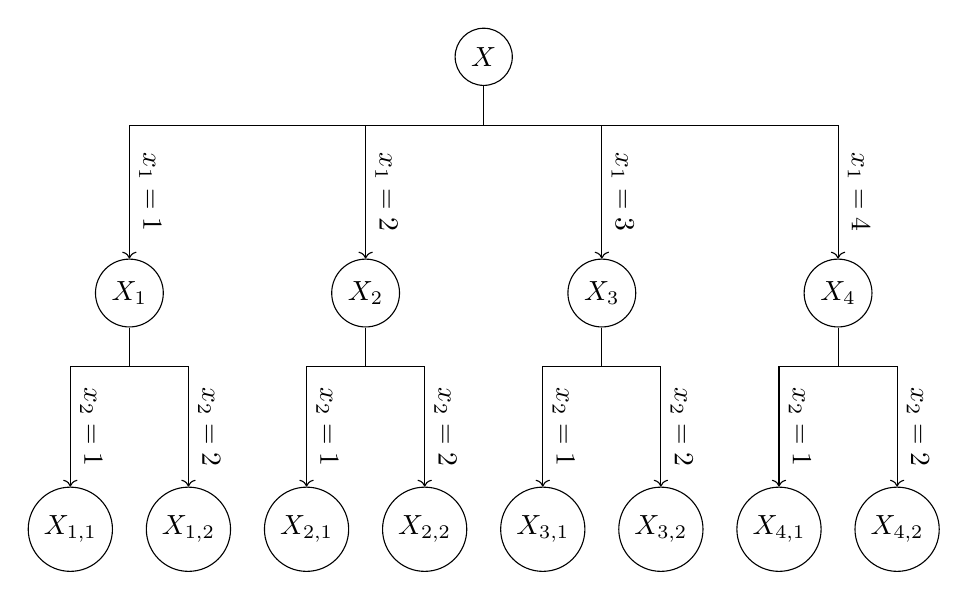
\begin{tikzpicture}[every child node/.style={circle,draw},level 1/.style={sibling distance=3cm},level 2/.style={sibling distance=1.5cm}, level distance = 3cm,edge from parent path={
(\tikzparentnode.south) |-   % Start from parent
++(0,-5mm) -|
    %($(\tikzparentnode.south)-(0,1mm)$) -|
%($(\tikzparentnode)!0.5!(\tikzchildnode)$) -| % make an ortho line to mid point
(\tikzchildnode.north)}]
        \node[circle,draw] (X) {$X$} 
	    child { node {$X_1$}
        	child { node {$X_{1,1}$} edge from parent [->] node (x2) [near end,above,sloped] {$x_2=1$} }
        	child { node {$X_{1,2}$} edge from parent [->] node (x2) [near end,above,sloped] {$x_2=2$} }
        	edge from parent [->] node [near end,above,sloped] (x1) {$x_1=1$}
            }
            child { node {$X_2$}
        	child { node {$X_{2,1}$} edge from parent [->] node [near end,above,sloped] {$x_2=1$} }
        	child { node {$X_{2,2}$} edge from parent [->] node [near end,above,sloped] {$x_2=2$} }
        	edge from parent [->] node [near end,above,sloped] {$x_1=2$}
            }
            child { node {$X_3$}
        	child { node {$X_{3,1}$} edge from parent [->] node [near end,above,sloped] {$x_2=1$} }
        	child { node {$X_{3,2}$} edge from parent [->] node [near end,above,sloped] {$x_2=2$} }
        	edge from parent [->] node [near end,above,sloped] {$x_1=3$}
            }
	    child { node {$X_4$}
        	child { node {$X_{4,1}$} edge from parent [->] node [near end,above,sloped] {$x_2=1$} }
        	child { node {$X_{4,2}$} edge from parent [->] node [near end,above,sloped] {$x_2=2$} }
        	edge from parent [->] node [near end,above,sloped] {$x_1=4$}
            }
            ;
	%\node[left = of x2] (x2_label) {$x_2=$};
	%\node at (x2_label |- x1) {$x_1=$};
	% \node[left = of x1 -| x2] {$x_1=$};
    \end{tikzpicture}
    \caption{Enumeration of all possible assignments for the integer variables of the example MILP problem of Eq. \eqref{eq:example-milp}, assuming lower and upper bounds are known. Leaf nodes contain the sets resulting from fixing the assignments, such that $X=X_1\cup \ldots\cup X_8$.}
    \label{fig:naive-tree-example-milp}
\end{figure}

The complete enumeration strategy for decomposing $X=X_1\cup \ldots\cup X_K$ implies that every $z^{k}=\min\{\bm{c}^{T}\bm{x} : \bm{x}\in X_k\}$ problem is an LP.
Therefore, once a leaf node is reached, it is possible to compute an optimal solution in polynomial time.

However, it is easy to see that complete enumeration of the integer assignments is not a viable option even for problems of moderate size.
Instead of searching on the complete tree of integer assignments, the branch-and-bound algorithm implements a guided exploration that ignores (or \emph{prunes}) entire branches of the tree based on upper and lower bounds of the problems associated to the decomposition of $X$.
To see this, first take a decomposition  $X=X_1\cup \ldots\cup X_K$ with $\bm{x}^k$ and $z^k$ as previously, and let $\underline{z}^{k}$ and $\overline{z}^{k}$ be lower and upper bounds (resp.) for every $z^{k}$.
Then, $\underline{z}=\min_k \underline{z}^{k}$ and $\overline{z}=\min_k \overline{z}^{k}$ are lower and upper bounds (resp.) for $z$.
Finally, if $\underline{z}^{k} \ge \overline{z}$ for a given $k$, then the optimal solution will not come from $X_k$, which implies that there is no need to explore the tree beyond $X_k$, i.e., that entire branch can be pruned. 

Again on the example MILP problem of \eqref{eq:example-milp}, suppose the LP relaxation of the problem was solved, which resulted in a lower bound $\underline{z}=2.5$.
Then, a decomposition based on variable $x_2$ was made, such that $X=X_1\cup X_2$, with $X_k = \left\{ \bm{x} : A\bm{x}\le \bm{b}, x_2 = k \right\}$.
The LP relaxation associated to each $X_k$ resulted in lower and upper bounds as denoted in Fig.~\ref{fig:pruning-example-milp}.
Because the lower bound of the problem associated to $X_1$ is greater than the upper bound of the problem associated to $X_2$, the optimal solution is definitely not in $X_1$, so this branch of the tree can be pruned.
Beyond that, the optimal solution of the LP relaxation from $X_1$ is already an integer solution, so no further decomposition is necessary. 

\begin{figure}[h]
    \centering
    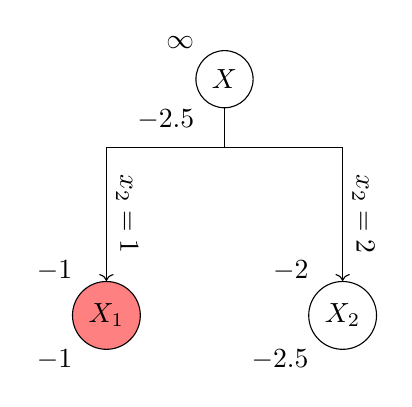
\begin{tikzpicture}[every child node/.style={circle,draw},level 1/.style={sibling distance=3cm},level 2/.style={sibling distance=1.5cm}, level distance = 3cm,edge from parent path={
(\tikzparentnode.south) |-   % Start from parent
++(0,-5mm) -|
    %($(\tikzparentnode.south)-(0,1mm)$) -|
%($(\tikzparentnode)!0.5!(\tikzchildnode)$) -| % make an ortho line to mid point
(\tikzchildnode.north)}]
        \node[circle,draw] (X) {$X$} 
	    child { node[fill=red!50] (X1) {$X_1$}
        	edge from parent [->] node [near end,above,sloped] (x1) {$x_2=1$}
            }
            child { node (X2) {$X_2$}
        	edge from parent [->] node [near end,above,sloped] {$x_2=2$}
            }
            ;
	\node[below left = 0cm of X] {$-2.5$} ;
	\node[above left = 0cm of X] {$\infty$} ;
	\node[below left = 0cm of X1] {$-1$} ;
	\node[above left = 0cm of X1] {$-1$} ;
	\node[below left = 0cm of X2] {$-2.5$} ;
	\node[above left = 0cm of X2] {$-2$} ;
	%\node[left = of x2] (x2_label) {$x_2=$};
	%\node at (x2_label |- x1) {$x_1=$};
	% \node[left = of x1 -| x2] {$x_1=$};
    \end{tikzpicture}
    \caption{Example of tree exploration with MILP problem of Eq. \eqref{eq:example-milp}. Associated upper (resp. lower) bounds are illustrated at the top (resp. bottom) left of each node. Node of set $X_1$ is painted red to indicate it is pruned based on the bounds from $X_2$.}
    \label{fig:pruning-example-milp}
\end{figure}



% As Fig.~\ref{fig:milp-example} illustrates, the optimal solutions to this problem are $\bm{x}^{*} \in \left\{ (2,2),(3,2) \right\} $, whereas the optimal solution of its LP relaxation is $(2.5, 2.5)$. 






The main idea behind the branch-and-bound algorithm is to ignore the integrality constraints of the MILP problem, solve the resulting LP, and hope that the solution has the necessary integer components~\cite{vanderbeiLinearProgrammingFoundations1998}.
If the LP relaxation\footnote{The linear programming problem obtained by ignoring the integrality constraints of an MILP is called its \emph{LP relaxation}.} of an MILP problem has an optimal solution that respects the integrality constraints, than that solution is also optimal for the original problem.
% integer solutions are naturally occuring to the LP problem on the convex hull of integer solutions for an MILP
% this is easy to see, as optimal solutions (if they exist) to LPs are always at the vertices of its feasible region (which is a polytope) and the vertices of the convex hull of an MILP all respect the original integrality constraints
However, that is not always the case.
As an example, take the MILP problem

\begin{figure}[h]
    \centering
    \includegraphics{pictures/milp_example_feasible_region.pdf}
    \caption{Feasible region of example MILP problem \eqref{eq:example-milp}. Dashed lines represent the feasible region of the LP relaxation.}
    \label{fig:milp-example}
\end{figure}

A naïve approach is to round the solution of the LP relaxation to the nearest integer value on the variables that violate the integrality constraints.
This strategy, however, might not even result in feasible solutions to the LP relaxation.
Note that an optimal solution to an LP is at a vertex of its feasible region, and, thus, a naïve deviation can result in an infeasible solution.

One way to guarantee that the solution to the LP relaxation will be the optimal solution to the MILP problem is to constrain the feasible region of the LP to be the \emph{convex hull} of $X$.
In other words, given an MILP problem such as in \eqref{eq:general-milp}, the solution to the LP problem
\begin{align*}
    \min_{\bm{x}} \quad & \bm{c}^{T}\bm{x} \\
    \textrm{s.t.} \quad & \bm{x}\in \conv(X) \times  \R^{n+p}
\end{align*}
is guaranteed to be the optimal solution to the original problem.



\subsection{Heuristics}

\subsection{Matheuristics}


	%% chapters/chapter_2.tex
%%
%% Copyright 2017 Evandro Coan
%% Copyright 2012-2014 by abnTeX2 group at http://abntex2.googlecode.com/
%%
%% This work may be distributed and/or modified under the
%% conditions of the LaTeX Project Public License, either version 1.3
%% of this license or (at your option) any later version.
%% The latest version of this license is in
%%   http://www.latex-project.org/lppl.txt
%% and version 1.3 or later is part of all distributions of LaTeX
%% version 2005/12/01 or later.
%%
%% This work has the LPPL maintenance status `maintained'.
%%
%% The Current Maintainer of this work is the Evandro Coan.
%%
%% The last Maintainer of this work was the abnTeX2 team, led
%% by Lauro César Araujo. Further information are available on
%% https://www.abntex.net.br/
%%
%% This work consists of a bunch of files. But originally there were 2 files
%% which are renamed as follows:
%% Deleted the `abntex2-modelo-img-marca.pdf`
%% Renamed the `abntex2-modelo-include-comandos.tex, v-1.9.2 laurocesar` to `chapters/chapter_1.tex`
%%
% ---
% Este capítulo, utilizado por diferentes exemplos do abnTeX2, ilustra o uso de
% comandos do abnTeX2 e de LaTeX.
% ---

% The \phantomsection command is needed to create a link to a place in the document that is not a
% figure, equation, table, section, subsection, chapter, etc.
% https://tex.stackexchange.com/questions/44088/when-do-i-need-to-invoke-phantomsection
\phantomsection

% https://tex.stackexchange.com/questions/5076/is-it-possible-to-keep-my-translation-together-with-original-text
\chapter{Deep Learning}\label{chap:deep-learning}

The advent of deep learning has revolutionized numerous fields, offering unprecedented capabilities in pattern recognition, decision-making, and problem-solving~\cite{Goodfellow-et-al-2016}.
In the realm of combinatorial optimization, particularly MILP, traditional methods often encounter computational bottlenecks when solving large-scale instances.
However, recent strides in deep learning have opened up exciting avenues for developing effective primal heuristics.
This chapter delves into the background of deep learning, focusing on the fundamental principles of supervised learning and neural network architectures.
The understanding of such concepts is essential for exploring the design and implementation of deep-learning-based solution prediction models tailored to MILP instances.


\section{Supervised Learning}

Supervised learning can be seen as the problem of finding a function that best associates inputs $x$ to outputs $y$ given a \emph{training set} with finitely many examples of such inputs and outputs~\cite{Goodfellow-et-al-2016}.
Although the machine learning area has attracted plenty of attention in the last decade, this learning problem is not new.
In fact, the core concepts were already established in the 1960s and 1970s~\cite{vapnikNatureStatisticalLearning2000}.
This section's approach to supervised learning will be that of statistical learning theory, based on \citeonline{vapnikNatureStatisticalLearning2000}, but with a more modern notation, derived from pattern recognition~\cite{bishopPatternRecognitionMachine2006,hastieElementsStatisticalLearning2009}.

To be more precise, supervised learning will be defined here as a problem of estimating a function that minimizes the risk.
Let $\mathcal{X}$ and $\mathcal{Y}$ be the input and output space, and $\mathcal{P}$ be a joint probability distribution over $\mathcal{X}\times \mathcal{Y}$.
To evaluate a function $f: \mathcal{X} \longrightarrow \mathcal{Y}$ with respect to its capacity to perform the right association between an input $x\in \mathcal{X}$ and an output $y\in \mathcal{Y}$, one measure's the discrepancy, or the \emph{loss}, $\ell(y,f(x))$.
In this context, the \emph{risk} associated to $f$ over the joint distribution $\mathcal{P}$ is the expected value of the loss function, or \[
    R(\mathcal{P},f) = \int_{\mathcal{X}\times \mathcal{Y}} \ell(y,f(x))\mathcal{P}(x,y)
    %R(f) = \mathbb{E}_{(x,y)\sim \mathcal{P}} \ell(y,f(x))
.\] 

The machine learning paradigm is that the joint probability function is fixed, but unknown, and one only has access to a finite number of samples~\cite{vapnikNatureStatisticalLearning2000}.
This idea is best represented through a \emph{dataset}, which is a finite set $\mathcal{D}$ of independent and identically distributed (i.i.d.) samples drawn according to $\mathcal{P}$.
In this context, the \emph{empirical risk} associated to a function $f$ over a dataset $\mathcal{D}$ is \[
    R_\textrm{emp}(\mathcal{D},f) = \frac{1}{|\mathcal{D}|} \sum_{(x,y)\in \mathcal{D}} \ell(y, f(x))
.\]

In this work, it is considered that the function to be estimated is chosen from a \emph{parametric model}\footnotemark, which is a family of functions $f: \mathcal{X}\times \Theta \longrightarrow \mathcal{Y}$ defined over a parameter space $\Theta$.
\footnotetext{This is in contrast to non-parametric models, whose functions' parameters are defined in terms of the dataset~\cite{murphyMachineLearningProbabilistic2013}.}
The problem then becomes that of finding a parameter vector that minimizes the empirical risk from a dataset $\mathcal{D}$, or \emph{fitting} a model to a dataset, denoted \[
\min_{\theta \in  \Theta} \mathcal{L}(\theta)
,\] where \[
    \mathcal{L}(\theta) = \frac{1}{|\mathcal{D}|} \sum_{(x,y)\in \mathcal{D}} \ell(y, f(x;\theta))
\] is an alternate, commonly found notation for the empirical risk, which often carries the name \emph{cost function}~\cite{murphyMachineLearningProbabilistic2013,bengioMachineLearningCombinatorial2021}.
Both "empirical risk" and "cost function" will be used interchangeably throughout this dissertation, although the former has a stronger connection to learning theory, while the latter is more related to practical matters.

A supervised learning algorithm is essentially an algorithm to optimize a cost function given a model and a dataset.
In fact, it is possible to define a supervised learning algorithm as a simple recipe: "combine a specification of a dataset, a cost function, an optimization procedure and a model"~\cite{bengioMachineLearningCombinatorial2021}.
Many different algorithms exist that are suitable for different components of this recipe.
For example, there are algorithms particular to decision tree models~\cite{breimanClassificationRegressionTrees2017}.
The least squares algorithm (used in the example of Section~\ref{sec:generalization-overfitting}) can be seen as a supervised learning algorithm for polynomial models given and the squared error loss function.

\subsection{Generalization and overfitting}\label{sec:generalization-overfitting}

Blindly minimizing the empirical risk can lead to a problem named \emph{overfitting}.
Overfitting happens when the empirical risk does not reflect the true risk, that is, when a function is \emph{fit} for the dataset, but not for the underlying data distribution.

This concept is best understood through an example.
Suppose $\mathcal{X},\mathcal{Y}\subseteq\R$ and that a dataset $\mathcal{D}$ with 40 i.i.d. samples is obtained such as illustrated in Fig.~\ref{fig:overfitting-example}.
It is desired to find a function that minimizes the risk measured through the squared error loss \[
    \ell(y,f(x)) = (y-f(x))^2
.\] 
The models $f_1,f_2,f_3$ are polynomials of degree 1, 3, and 15, whose parameters are the weights of the polynomials.
These models are adjusted using least squares algorithm, resulting in parameter vectors $\theta_1^*,\theta_2^*,\theta_3^*$ that achieve a global minimum of the empirical risk with their respective models.
The performance of these models is illustrated in Fig.~\ref{fig:overfitting-example}.

Note that model $f_3$ achieves the lowest empirical risk on $\mathcal{D}$.
However, $f_2$ is the one that seems to best associates inputs to outputs, considering a visual intuition of the underlying data distribution.
One could say that $f_3$ is \emph{too complex} for the underlying distribution, which leads to it being more tightly adjusted to the noise present in the dataset rather than on the underlying data distribution~\cite{murphyMachineLearningProbabilistic2013}.
On the other hand of the spectrum is the $f_1$ model, which is not complex enough to model the desired behavior.
While $f_3$ is overfitting the data, $f_1$ is underfitting it.

\begin{figure}[h]
    \centering
    \includegraphics{pictures/overfitting.pdf}
    \caption{Example of overfitting. The three models shown ($f_1,f_2,f_3$) are polynomials of degree 1, 3 and 10 adjusted to the dataset $\mathcal{D}$. The optimal parameter vectors $\theta_1^*,\theta_2^*$ and $\theta_3^*$ were adjusted using a least squares algorithm. The empirical risks are $\mathcal{L}(\theta_1^*)=79.67$, $\mathcal{L}(\theta_2^*)=7.64$, and $\mathcal{L}(\theta_3^*)=5.48$.}
    \label{fig:overfitting-example}
\end{figure}

The level of overfitting that a function $f$ presents could be determined through the \emph{generalization gap}, which is the difference between the empirical risk and the true risk $R(\mathcal{P},f) - R_\textrm{emp}(\mathcal{D},f)$~\cite{murphyMachineLearningProbabilistic2013}.
More specifically, a function can be said to overfit the dataset if it has a high generalization gap.
As the underlying distribution $\mathcal{P}$ is not known, the generalization gap is approximated by \emph{splitting} the dataset $\mathcal{D}$ into a training set $\mathcal{D}_\textrm{train}$ and a test set $\mathcal{D}_\textrm{test}$.
The idea is that the parameters of the model are adjusted according to the empirical risk of $\mathcal{D}_\textrm{train}$, while $\mathcal{D}_\textrm{test}$ is reserved for estimating the true risk, also called \emph{generalization error}.
This way, the resulting function cannot be overfitted to $\mathcal{D}_\textrm{test}$, which is kept as an untouched source of information of the underlying distribution.
Finally, the generalization gap can be estimated as  \[
    R_\textrm{emp}(\mathcal{D}_\textrm{test},f) - R_\textrm{emp}(\mathcal{D}_\textrm{train},f)
.\] 

\subsection{Hyperparameter optimization}

In practice, the dataset $\mathcal{D}$ is partitioned into three sets, as a validation set $\mathcal{D}_\textrm{val}$ is necessary for \emph{hyperparameter optimization}.

% See Bengio et al., Ch. 5.3

\section{Neural Networks}

\subsection{Gradient-based learning}

% See Bengio et al., Ch. 6.2

\subsection{Graph Neural Networks}




	\part{Materials and Methods}{materials-and-methods}

	
% The \phantomsection command is needed to create a link to a place in the document that is not a
% figure, equation, table, section, subsection, chapter, etc.
% https://tex.stackexchange.com/questions/44088/when-do-i-need-to-invoke-phantomsection
\phantomsection

\chapter{Solution Prediction Models for MILP Problems}\label{chap:solution-prediction}


This chapter introduces the methods available for training deep learning models for predicting solutions of MILP problems.
The ability to efficiently predict solutions plays a pivotal role in the development of learning-based heuristics.
In other words, this chapter is a bridge between Chapters \ref{chap:integer-programming} and \ref{chap:deep-learning} with a focus on (mat)heuristics.

This chapter begins by discussing the process of embedding of MILP problems, which involves transforming problem instances into a suitable format for deep learning models.
Within this context, feature engineering and graph approaches are explored to represent the intricate relationships between the components of MILP problems.
Moving forwards, the methodologies employed in training deep learning models fed with embeddings of MILP problem instances are presented, highlighting the challenges and opportunities posed by the availability of multiple feasible solutions.
The chapter ends with the approaches one can use to create primal (mat)heuristics from solution prediction models.


\section{Embedding Optimization Problems}

% TODO: see SatGNN paper

The first requirement that needs to be satisfied for training deep learning models to predict solutions to MILP problems is to be able to feed instances of MILP problems to such models.
For this, it is necessary to convert an instance to a numerical format that the model can handle.

Naturally, an instance can be specified by a tuple $\left( \bm{c}, \bm{b}, A, n \right)$, as discussed in Sec.~\ref{sec:milp-definition}, which could be vectorized an be fed to a vanilla NN.
This form of embedding, which is going to be referred to as \emph{naïve} embedding, has several shortcomings.
First, it does not represent the \emph{symmetries} of the formulation, which are operations applied to the parameters that do not alter its solutions.
For example, changing the order of the constraints, which can be seen as permutations of rows of $\left[ A\, | \,\bm{b} \right] $, does not affect in any way the feasible space nor the objectives associated to feasible solutions, but generates different embeddings.

Furthermore, the naïve embedding can easily be an over-parametrization of the instance distribution, which often are sampled from a lower-dimensional space.
For example, take the MILP formulation of the TSP by \citeonline{millerIntegerProgrammingFormulation1960}
\begin{align*}
    \min_{\bm{u},\bm{x}} \quad & \sum_{\substack{i,j=0 \\ i\neq j}}^{n} d_{ij} x_{ij} & \\
    \textrm{s.t.} \quad & \sum_{\substack{i=0\\i\neq j}}^{n} x_{ij} = 1, &\, j=1,\ldots,n \\
			& \sum_{\substack{j=0\\j\neq i}}^{n} x_{ij} = 1, &\, i=1,\ldots,n \\
			& u_i - u_j + n \cdot x_{ij} \le n - 1, &\, i,j=1,\ldots,n,\, i\neq j\\
			& x_{ij} \in \left\{ 0,1 \right\}, &\, i,j=0,\ldots,n  \\
			& \bm{u} \in \R^{n} &
\end{align*}
and suppose one wants to solve it for instance $I\in \mathcal{I}$ over the same graph but with varying edge costs $d_{ij}$.
Of course, embedding such instances naïvely would encode all the static parameters of the constraints, i.e., the information that does not change between the instances of interest, which do not carry relevant information for the model.


\subsection{Feature Engineering}

One way to mitigate the shortcomings of the naïve embedding is to extract \emph{features} that well represent the instance with respect to their solutions.
This approach is based on the hypothesis that, for a given application, the instances are sampled from a lower-dimensional space, i.e., that there exists a mapping $g: X\subseteq\R^{d} \longrightarrow \mathcal{I}$ that associates features $x\in X$ to instances $I\in \mathcal{I}$, and that $d$ is significantly smaller than the number of parameters (e.g., from the naïve embedding).

Continuing with the TSP example from above, suppose that the goal is to solve the TSP for a given city (which fixes the graph over which the tours are to be found) but with different traffic conditions and, therefore, different edge costs $d_{ij}$.
The cost vector $\bm{c}$ (which is a vectorization of the $d_{ij}$ parameters) can be said a feature vector for the instances, but calling this feature engineering would be controversial statement.
However, one could investigate what are the variables that influence the traffic conditions, e.g., hour of the day, day of the week, gas price, weather.
Ideally, then, it would be possible to use these variables to define a feature space $X$, such that a mapping $g: X \longrightarrow \mathcal{I}$ exists, and train models that are fed with $x\in X$.
Note that, in practice, one does not need to know $g$ to be able to train a deep learning model, only its \emph{inverse}, i.e., it is only necessary to compute features given instances, and assume that the inverse is possible.

Embedding MILP problem instances as feature vectors is an approach suitable for NNs, as they require vector-valued inputs.
However, there is an underlying restriction that is a fixed number of features.
Although it seems natural, it is not always the case that all instances of a problem have the same number of variables or constraints.
If in the TSP example above the underlying graph changes over the instance space, then the instances will have varying numbers of variables and constraints.
In the naïve embedding, this translates directly to vectors of varying size, which are not directly suitable for NNs.
To generate features that are suitable for NNs even when the instances have varying size, the feature engineer must be able to translate the process that changes the size of the instances into a fixed number of features, which is not always easy or even feasible.

\subsection{Graph Embedding}

A well-used approach in the intersection between deep learning and combinatorial optimization is to embed MILP problem instances is through bipartite graphs~\cite{gasseExactCombinatorialOptimization2019,nairSolvingMixedInteger2021,dingAcceleratingPrimalSolution2020,khalilMIPGNNDataDrivenFramework2022,hanGNNGuidedPredictandSearchFramework2023}.
Any instance of an LP problem can be represented as a weighted bipartite graph.
Consider the problem
\begin{equation}\label{eq:example-lp-graph}
\begin{aligned}
    \max_{\bm{x}} & \quad \bm{c}^T \bm{x} \\
    \text{s.t.:} & \quad A\bm{x} \le\bm{b} 
,\end{aligned}
\end{equation}
where $\bm{x}\in X \subseteq\mathbb{R}^n$ and $\bm{b}\in \mathbb{R}^m$.
It is possible to build a bipartite graph $G=(V_{\textrm{var}}\cup V_{\textrm{con}}, E)$, in which $v_{\textrm{con},i}\in V_{\textrm{con}}$ is the node associated to the $i$-th constraint, $v_{\textrm{var},j}\in V_{\textrm{var}}$ is the node associated to $x_j$, and $E=\{(v_{{\rm con},i},v_{{\rm var},j}) : A_{i,j} \neq 0\}$.
Furthermore, a weight function $w: V_{\textrm{var}}\cup V_\textrm{con}\cup E \longrightarrow \R$ such that $w(v_{\textrm{var},i}) = c_j$, $w(v_{\textrm{con},j}) = b_j$, and $w(e_{i,j}=(v_{\textrm{con},i},v_{\textrm{var},j})) = A_{i,j}$, renders the weighted graph $(G,w)$ a complete representation of any instance of the LP, i.e., the original LP instance can be reconstructed using solely the information in such weighted graph.

The extension to MILP problems requires solely the distinction between continuous and integer variables.
This can be done, for example, by extending the weight function to a vector-valued function such that $w(v_{\textrm{var},j}) = (c_j,0)$ if the $j$-th variable is continuous or $w(v_{\textrm{var},j}) = (c_j,1)$ if $x_j$ is an integer variable.
In practice, however, the graph fed to a GNN is usually "weighted" with feature vectors $\bm{h}_v^{(0)}, \forall v\in V$ of arbitrary size, as seen in Sec.~\ref{sec:gnns}.
In other words, the information contained in the weights (feature vectors) provided to the network is a design choice.
It can contain the weights described above, but many other features might also help the model learn the graph-related task (see, for example, \citeonline{gasseExactCombinatorialOptimization2019} and \citeonline{nairSolvingMixedInteger2021}).

The graph embedding is perfectly suitable for GNNs.
In comparison to the feature engineering approach, the graph embedding requires no effort from an human expert, and provides an effective result in terms of representation power and scalability.
First, because the resulting graph contains all of the information present in the instance while being invariant to constraint and variable permutations.
On top of that, the size of the GNN does no scale with the size of the graph, but solely with the dimension of the weight (feature vector) associated to each node.


\section{Training Under Supervision}

\subsection{Multiple Targets}

\section{Learning-based Heuristics}\label{sec:learning-based-heuristics}

\subsection{Early-fixing Variable Assignments}

\subsection{Trust-region}

\subsection{Warm-starting MILP Solvers}


	
% The \phantomsection command is needed to create a link to a place in the document that is not a
% figure, equation, table, section, subsection, chapter, etc.
% https://tex.stackexchange.com/questions/44088/when-do-i-need-to-invoke-phantomsection
\phantomsection

\chapter{Offline Nanosatellite Task Scheduling}\label{chap:onts}

This chapter delves into the application area of the experiments conducted for this dissertation, specifically focusing on the Offline Nanosatellite Task Scheduling (ONTS) problem.
Over the past decade, nanosatellites have gained significant attention from both industry and academia, primarily due to their cost-effective development and launch processes~\cite{shiromaCubeSatsBrightFuture2011,luciaComputationalNanosatelliteConstellations2021,nagelNanosatellitesAppliedOptical2020,saeedCubeSatCommunicationsRecent2020}.
Despite these advantages, the limited computational and energy resources of nanosatellites present substantial challenges in mission planning.
Effective task scheduling is essential to optimize resource utilization, enhance data quality, and ensure mission success, thereby securing a return on investment.

The ONTS problem is critical for the efficient development, deployment, and operation of nanosatellites.
From launch to disposal, the ONTS problem must be solved repeatedly.
At every communication window, new schedules must be generated and deployed, and the optimal schedule is determined by an iterative procedure, exploring different sets of tasks to be performed in the schedule's timespan.
Given a nanosatellite and a collection of tasks, determining the schedule with maximum QoS is a combinatorial problem.
Mathematical formulations have been proposed for this problem, from Integer Programming (IP)~\cite{rigoTaskSchedulingOptimal2021} to Mixed Integer Linear Programming (MILP)~\cite{rigoNanosatelliteTaskScheduling2021,semanEnergyAwareTaskScheduling2022} and Continuous-Time techniques~\cite{camponogaraContinuoustimeFormulationOptimal2022}.
However, the NP-hard nature of the problem renders multiple executions of the optimization algorithms (e.g., for different task configurations) within the timespan of a communication window an efficiency challenge.

The following section will present the problem statement with a description of the factors that are taken into consideration.
Then, the MILP formulation of the problem, proposed by \citeonline{rigoNanosatelliteTaskScheduling2021}, is presented, which will be the basis for the experiments presented in Part~\ref{experiments-and-results}.

% The instances to be solved share common features.
% Beyond the problem structure, which remains unaltered, tasks, orbit information, and battery capacity can be understood as being randomly drawn from an unknown distribution at every communication window.
% This setup fits the context of primal heuristics based on 
% 
% It involves determining an optimal schedule for task execution that maximizes Quality-of-Service (QoS).
% This requires careful consideration of various factors, including task priority, minimum and maximum activation events, execution time frames, periods, and execution windows.
% Additionally, the constraints imposed by the satellite's power resources and the complexities of energy harvesting and management systems must be addressed.
% By solving the ONTS problem, we can significantly improve the operational efficiency and effectiveness of nanosatellite missions, ensuring their success and sustainability.


\section{Problem Statement}

Nanosatellite scheduling problems involve making decisions regarding the start and finish times of each task.
These tasks often require periodic execution and must be scheduled during specific moments along the satellite's orbit.
In addition to temporal constraints, energy availability throughout the orbit is a crucial resource that must be taken into account.
Figure \ref{fig:example-scheduling} illustrates an example of optimal scheduling, where each job is represented by a different color, and the activation and deactivation of tasks are depicted as steps in the signal sequence.

\begin{figure}[h]
    \centering
    \includegraphics{schedule_example.pdf}
    \caption{Illustration of an optimum schedule for 9 tasks on a horizon of 125 time steps. Each color represents the executions of a different task.}
    \label{fig:example-scheduling}
\end{figure}

Effective scheduling must incorporate energy management to ensure that tasks do not consume more energy than the system can provide, thereby preventing the battery from depleting before the mission concludes.
Energy management is particularly challenging because the nanosatellite relies on solar panels for power.
The energy availability is influenced by the nanosatellite's attitude, which affects the orientation of the solar panels, and its trajectory relative to Earth's shadow, as depicted in Figure \ref{fig:onts-orbit}.
On top of that, the shared energy resources steps up the problem complexity, as each task's activation must be determined while taking into consideration the other tasks.

\begin{figure}[h]
    \centering
    \includegraphics[width=0.5\textwidth]{onts_orbit.png}
    \caption{Illustration of a nanosatellite's orbit around Earth. Image from \citeonline{rigoBranchandpriceAlgorithmNanosatellite2022}.}
    \label{fig:onts-orbit}
\end{figure}


\section{MILP Problem}

The formulation presented here was proposed by \citeonline{rigoTaskSchedulingOptimal2021} and the reader is advised to refer to the original work for further details.

Given a set $\mathcal{J}=\{1,...,J\}$ of tasks (or jobs), and a set $\mathcal{T}=\{1,...,T\}$ of time units of the scheduling horizon, let variables $x_{j,t}$ represent the allocation of task $j$ at time $t$, $\forall j\in \mathcal{J}, \forall t\in \mathcal{T}$.
Naturally, each $x_{j,t}$ is a binary variables, in which value $1$ indicates that task $j$ is scheduled to be in execution at time $t$.
When convenient, these variables will be represented as a vector \[
    % \bm{x}=(x_{1,1},\ldots,x_{1,T},\ldots,x_{J,1},\ldots,x_{J,T})
    \bm{x} = \left( x_{j,t} \right)_{\substack{j=1,\ldots,J\\ t=1,\ldots,T}}
,\] which is a notation also used for other variables and parameters.

Every task $j$ has an associated priority $u_j > 0$, such that the mission's QoS is defined as
\begin{equation}\label{eq:qos}
    {\rm QoS}(\bm{x};\bm{u}) = \sum_{j=1}^{J} \sum_{t=1}^{T} {u}_{j} x_{j,t}
.\end{equation}
As mentioned previously, the goal of the optimization problem is to find a schedule that maximizes the QoS.

Auxiliary variables $\phi_{j,t}$ are defined for every $j\in \mathcal{J}$ and $t\in \mathcal{T}$, which represent the startup of the task, i.e., $\phi_{j,t} = 1$ indicates that task $j$ is not running at time $t-1$ but its execution is started at time $t$.
The behavior of these auxiliary variables is ensured by
\begin{equation}\label{eq:phi-constraints}
    \begin{aligned}
	& \phi_{j,t} \geq x_{j,t}, &~\forall j\in\mathcal{J},\, t = 1  \\
        & \phi_{j,t} \geq x_{j,t} - x_{j,(t-1)}, &~\forall j\in\mathcal{J}, \,\forall t\in\mathcal{T}: t > 1   \\
        & \phi_{j,t} \leq x_{j,t}, &~\forall j\in\mathcal{J}, \,\forall t\in\mathcal{T}   \\
        & \phi_{j,t} \leq 2 - x_{j,t} - x_{j,(t-1)}, &~\forall j\in\mathcal{J}, \,\forall t\in\mathcal{T}: t > 1
    .\end{aligned}
\end{equation}

The multiple requirements of each task are ensured by a series of constraints.
Each task $j$ may run only during a specified time window delimited by $w_{j}^{\text{min}}$ and $w_{j}^{\text{max}}$, which is imposed by
\begin{equation}\label{eq:window-constraints}
    \begin{aligned}
        &\sum_{t=1}^{\textcolor{black}{w^{\min}_{j}}} x_{j,t} = 0,  & \forall j\in\mathcal{J} \\
        &\sum_{t=w^{\max}_{j}+1}^{T} x_{j,t} = 0, & \forall j\in\mathcal{J}
    .\end{aligned}
\end{equation}
Such constraints can be used to force a task to be executed when the nanosatellite is passing over a predetermined region.

To limit continuous executions, a task $j$ is constrained to run without interruption for least $t_j^{\text{min}}$, and at most $t_j^{\text{max}}$ time steps, which is imposed by
\begin{equation}\label{eq:execution-gap-constraints}
    \begin{aligned}
        &\sum_{l=t}^{t+{t}^{\min}_{j}-1} x_{j,l} \geq {t}^{\min}_{j} \phi_{j,t},  &\forall t \in \{1,...,T-{t}^{\min}_{j} + 1\}, \forall j\in\mathcal{J} \\
        &\sum_{l=t}^{t+{t}^{\max}_{j}} x_{j,l} \leq {t}^{\max}_{j},  &\forall t \in \{1,...,T-{t}^{\max}_{j}\}, \forall j\in\mathcal{J}
    .\end{aligned}
\end{equation}
Complementary, and having in mind that the end of schedule is not the end of the nanosatellite life, the addition of constraint
\begin{equation}\label{eq:execution-end-constraints}
    \begin{aligned}
        &\sum_{l=t}^{T} x_{j,l} \geq (T - t + 1) \phi_{j,t},  & \forall t \in \{T-{t}^{\min}_{j} + 2,...,T\}, \forall j\in\mathcal{J}
    \end{aligned}
\end{equation}
enables the start of the execution of a task close to the end of the schedule horizon, and keep it running until the end.

For a task to be executed periodically, at least every $p_j^{\text{min}}$ time steps, and at most every $p_j^{\text{max}}$ time steps, the following constraints are added:
\begin{equation}\label{eq:prediodicity-constraints}
    \begin{aligned}
        &\sum_{l=t}^{t+{p}^{\min}_{j}-1} \phi_{j,l} \leq 1,   & \forall t \in \{1,...,T-{p}^{\min}_{j}+1\}, \forall j\in\mathcal{J}  \\
        & \sum_{l=t}^{t+{p}^{\max}_{j}-1} \phi_{j,l} \geq 1,  & \forall t \in \{1,...,T-{p}^{\max}_{j}+1\},  \forall j\in\mathcal{J} 
    .\end{aligned}
\end{equation}
On top of that, a task may be required to run multiple times over the planning horizon.
The constraints
\begin{equation}\label{eq:multiple-execs-constraints}
    \begin{aligned}
        &\sum_{t=1}^{T} \phi_{j,t} \geq {y}^{\min}_{j}, &\forall j\in\mathcal{J}   \\
        &\sum_{t=1}^{T} \phi_{j,t} \leq {y}^{\max}_{j}, &\forall j\in\mathcal{J}
    \end{aligned}
\end{equation}
are added to ensure at least $y_{j}^{\text{min}}$ and at most $y_j^{\text{max}}$ runs are performed for task $j$.

The energy-management restrictions are ensured through multiple constraints.
Given $r_t$, the power available from the solar panels at each time $t$, $q_j$, the power required by each task $j$, and $\gamma~V_{b}$, the maximum power the battery can provide, then
\begin{equation}\label{eq:power-consumption-constraints}
    \begin{aligned}
	&\sum_{j=1}^{J} q_{j} x_{j,t} \leq r_t + \gamma~V_{b}, & \forall t\in\mathcal{T}
    \end{aligned}
\end{equation}
limits the power consumption to realistic levels.
Auxiliary variables $b_t$ and $\text{SoC}_t$ represent, resp., the exceeding power and the State of Charge (SoC) over each time $t\in \mathcal{T}$.
Given $Q$, the battery capacity, and $e$, the discharge efficiency, the exceeding power is ensured by
\begin{equation}\label{eq:exceeding-power-constraints}
    \begin{aligned}
	& b_{t} = r_{t} - \sum_{j \in \mathcal{J}} q_{j} x_{j,t}, &  \forall t \in \mathcal{T}
    ,\end{aligned}
\end{equation}
while the SoC is ensured by
\begin{equation}\label{eq:SoC-constraints}
    \begin{aligned}
    &\text{SoC}_{t+1} = \text{SoC}_{t} + \frac{b_{t}~e}{60~Q~V_{b}}, & \forall t \in \mathcal{T}  \\
    &\text{SoC}_{t} \leq 1, & \forall t\in\mathcal{T}    \\
    &\text{SoC}_{t} \geq \rho, & \forall t\in\mathcal{T}
    ,\end{aligned}
\end{equation}
where $\rho$ is the allowed lower limit for the battery, which is usually greater than zero for safety purposes.

Finally, the ONTS problem is formulated as an MILP
\begin{equation}\label{eq:onts-milp}
\begin{aligned}
    \max_{\bm{x},\bm{\phi},\bm{\text{SoC}},\bm{b}} \quad & \eqref{eq:qos} \\
    \textrm{s.t.} \quad & (\ref{eq:phi-constraints} \text{--} \ref{eq:SoC-constraints}) \\
	    & x_{j,t}, \phi_{j,t} \in \left\{ 0,1 \right\} ,\quad \forall j\in \mathcal{J}, t\in \mathcal{T} \\
.\end{aligned} \tag{ONTS}
\end{equation}
Note that the constraints \eqref{eq:exceeding-power-constraints} and \eqref{eq:SoC-constraints} imply that the continuous variables $\bm{b}$ and $\bm{\text{SoC}}$ are uniquely determined by a given assignment for the binary variables $\bm{x}$ and $\bm{\phi}$.
Therefore, the problem can be reduced to finding an assignment $\bm{y}=(\bm{x},\bm{\phi}) \in \left\{ 0,1 \right\}^{n}$, where $n=2JT$.

Let $\mathcal{I}$ be the space of all MILP problems of the form \eqref{eq:onts-milp}.
Any instance $I\in \mathcal{I}$ is parameterized by $\pi_I = \left( \bm{u}, \bm{q}, \bm{y}^{\min}, \bm{y}^{\max}, \bm{t}^{\min}, \bm{t}^{\max}, \bm{p}^{\min}, \bm{p}^{\max}, \bm{w}^{\min}, \bm{w}^{\max}, \bm{r}, \rho, e, Q, \gamma, V_b \right) $, and, implicitly, by the number of tasks $J$ and the number of time units $T$.
Let $\Pi^{J,T}$ denote the space of parameter vectors as above, such that any instance $I\in \mathcal{I}$ can be uniquely determined by a parameter vector $\pi_{I}$ (given adequate $J$ and $T$).



	
% The \phantomsection command is needed to create a link to a place in the document that is not a
% figure, equation, table, section, subsection, chapter, etc.
% https://tex.stackexchange.com/questions/44088/when-do-i-need-to-invoke-phantomsection
\phantomsection

\chapter{Evaluation of Primal Heuristics}\label{chap:evaluation}

\section{Standard Evaluation Metrics}

\begin{itemize}
    \item Runtime
    \item GAP
    \item Infeasibility\%
\end{itemize}

\section{Area Under the Primal-dual Curve}

- add illustration of the backwards-filling scheme for fairness



	\part{Experiments and Results}\label{experiments-and-results}

	
% The \phantomsection command is needed to create a link to a place in the document that is not a
% figure, equation, table, section, subsection, chapter, etc.
% https://tex.stackexchange.com/questions/44088/when-do-i-need-to-invoke-phantomsection
\phantomsection

\chapter{Experiments}\label{chap:experiments}

To address the objective of this dissertation, experiments are conducted to evaluate learning-based primal heuristics for Mixed-Integer Linear Programming (MILP).
The ONTS problem (see Chap.~\ref{chap:onts}) serves as a realistic application to benchmark the selected techniques.

As discussed in Section~\ref{sec:onts-problem-statement}, during mission execution (with the nanosatellite in orbit), a new schedule must be generated during the communication window.
This involves optimizing multiple instances of the ONTS problem, given varying sets of tasks and updated nanosatellite information.
Each set of tasks is evaluated based on the resulting schedule, in an iterative process of including new tasks until scheduling becomes infeasible.
Therefore, during the communication window, quickly finding a good solution to a problem instance is more crucial than finding an optimal solution.
In other words, an efficient heuristic is crucial to allow for more iterations, which leads to a better set of tasks scheduled for execution.

The remaining of this chapter details the development and the experiments with the proposed learning-based heuristics for the ONTS problem.
This includes data acquisition, solution prediction model architecture, model training, and experiment setup.
Furthermore, the performance of the proposed learning-based heuristics is assessed on realistic instances of the ONTS problem.


\section{Data}

High-quality data is necessary both to train solution prediction models and to evaluate the proposed learning-based heuristics for the ONTS problem.
The datasets for both training and evaluation must be composed of instance-solution pairs, as discussed in Sec.~\ref{sec:training-solution-prediction}.
The quality of these instance-solution pairs is measured through their faithfulness, both the instance with respect to the true data distribution, and the solution with respect to the optimal.

\subsection{Instance space: the FloripaSat I mission}\label{sec:instance-space}

The instance space is defined from the parameters of the FloripaSat-I mission~\cite{marcelinoCriticalEmbeddedSystem2020}.
Their nanosatellite is in orbit at an altitude of 628 kilometers and an orbital period of 97.2 minutes.
The planning horizon is fixed at $T=125$ time slots, with one slot per minute, to account for a continuous scheduling, allowing for task executions that extend the communication window.
Any instance $I\in \mathcal{I}$ has either 9, 13, 18, 20, 22, or 24 tasks.

Once the orbit of the FloripaSat-I is stable and its received solar flux is constant, the power input vector $\bm{r}$ can be calculated deterministically from solar irradiance measurements as in \citeonline{morschfilhoComprehensiveAttitudeFormulation2020}.
Two years of solar irradiance data are used as a basis for the power input vectors of the instances in the instance space.
The set $R$ is used to denote all possible values of $\bm{r}$ from the historical data.
The other battery-related parameters (see Sec.~\ref{sec:onts-milp-formulation}) are fixed as 
\begin{align*}
    e &= 0.9 \\
    Q &= 5 \\
    \gamma &= 5 \\
    V_b &= 3.6 \\
    \rho &= 0.0
\end{align*}

The remaining parameters are constrained to ranges that match previous works in the area~\cite{rigoBranchandpriceAlgorithmNanosatellite2022,semanEnergyAwareTaskScheduling2022,rigoTaskSchedulingOptimal2021}.
Therefore, following the notation established in Sec.~\ref{sec:onts-milp-formulation}, the parameter space is defined as
\begin{equation}\label{eq:parameter-space}
\Pi = \bigcup_{\substack{J \in \left\{ 9,13,18,20,22,24 \right\} \\ T \in \left\{ 125 \right\} }} \Pi^{J,T}
,\end{equation}
where each $\Pi^{J,T}$ is a set of a parameter vectors \[
\pi_I= \left( \bm{u}, \bm{q}, \bm{y}^{\min}, \bm{y}^{\max}, \bm{t}^{\min}, \bm{t}^{\max}, \bm{p}^{\min}, \bm{p}^{\max}, \bm{w}^{\min}, \bm{w}^{\max}, \bm{r}, \rho, e, Q, \gamma, V_b \right) \in \Pi^{J,T}
\] such that
\begin{equation*}
\begin{aligned}
&\begin{rcases}
    & u_j \in [1, J] \\
	 & q_j \in [0.3, 2.5] \\
    	 & y_j^{\min} \in [1, \lceil T/45 \rceil] \\
    	 & y_j^{\max} \in [y_j^{\min}, \lceil T/15 \rceil] \\
    	 & t_j^{\min} \in [1, \lceil T/10 \rceil] \\
    	 & t_j^{\max} \in [t_j^{\min}, \lceil T/4 \rceil] \\
    	 & p_j^{\min} \in [t_j^{\min}, \lceil T/4 \rceil] \\
    	 & p_j^{\max} \in [p_j^{\min}, T] \\
    	 & w_j^{\min} \in [0, \lceil T/5 \rceil] \\
    	 & w_j^{\max} \in [\lfloor T-\lceil T/5 \rceil \rfloor, T]
\end{rcases} \forall j =1,\ldots,J \\
    &\quad \bm{r} \in R ,\, e = 0.9 ,\, Q = 5 ,\, \gamma = 5 ,\, V_b = 3.6 ,\, \rho = 0.0
.\end{aligned}
\end{equation*}
Finally, the input space is then defined from the parameter space, such that \[
    I\in \mathcal{I} \iff \pi_I \in \Pi 
.\] 


\subsection{Data acquisition}\label{sec:data-acquisition}

As historical data is not available for the ONTS problem, the dataset is built from randomly generated instances sampled uniformly from the instance space of the FloripaSat-I mission.
More precisely, the dataset is built with instances drawn uniformly from the instance space defined above.

As the addition of an element to the dataset requires a solution to the ONTS problem, the computational cost of building a large dataset with hard instances is very high.
To alleviate this cost, the training set is built solely with instances with fewer tasks, which are, on average, faster to solve than instances with many tasks.
However, the instances of interest are those with plenty of tasks, which are harder to solve in practice, and, thus, motivate the use of heuristics.
Therefore, the validation and test datasets are built from instances with many tasks, which are, on average, significantly harder to solve.
Table~\ref{tab:dataset} details the number of instances by size (number of tasks) in each dataset generated.

\begin{table}[h]
    \centering
    \caption{Number of instances by size in each dataset. The datasets were generated through Algorithm~\ref{alg:dataset-generation}.}
    \label{tab:dataset}
    \begin{tabular}{l | c | c | c}
    \toprule
    & Training & Validation & Test \\
    \midrule
    $J = 9$ & 200 & 0 & 0 \\
    $J = 13$ & 200 & 0 & 0 \\
    $J = 18$ & 200 & 0 & 0 \\
    $J = 20$ & 0 & 20 & 20 \\
    $J = 22$ & 0 & 20 & 20 \\
    $J = 24$ & 0 & 20 & 20 \\
    \midrule
    Total & 600 & 60 & 60 \\
    \bottomrule
    \end{tabular}
\end{table}

Distinguishing the size of the instances in each dataset allows for the construction of a large training set, which enables the models to properly learn the problem, while maintaining a challenging evaluation scenario.
On top of that, this approach also enables the evaluation of the generalization capabilities of the proposed solution prediction models and the derived learning-based heuristics.

The algorithm to generate the datasets is presented in Algorithm~\ref{alg:dataset-generation}.
Note that an instance is rejected if no feasible solution is found during the time budget or if the solver proves infeasibility.
As the time horizon is fixed, the algorithm is executed once for each number of tasks.
Similar to the parameter space definition \eqref{eq:parameter-space}, the resulting dataset can be described as
\begin{equation}\label{eq:dataset}
    \mathcal{D} = \bigcup_{\substack{J \in \left\{ 9,13,18,20,22,24 \right\} \\ T \in \left\{ 125 \right\} }}  \mathcal{D}^{(J,T)}
,\end{equation}
where each $\mathcal{D}^{(J,T)}$ is obtained through Algorithm~\ref{alg:dataset-generation}.
The algorithm is such that each element of the output dataset $(I,Z^\star_I) \in \mathcal{D}^{(J,T)}$ is composed of a \emph{feasible} instance $I$ sampled uniformly from the parameter space (see Eq.~\eqref{eq:parameter-space}) and deemed feasible by an MILP solver.
Furthermore, the accompanying set $Z^\star_I$ contains the best solutions found by the solver, which are necessary for training the model with multiple solutions as a target (see Sec. \ref{sec:multiple-targets}).

For our experiments, the algorithm was executed such that every new instance $I$ was solved using the SCIP solver~\cite{bestuzhevaSCIPOptimizationSuite2021} with a limited time budget of 5 minutes.
The best 500 solutions of each instance $I$ were recorded, i.e., for every $(I,Z^{*}) \in \mathcal{D}$, $|Z^{*}_I| = 500$.
Finally, the dataset is divided as $\mathcal{D} = \mathcal{D}_\textrm{train} \cup \mathcal{D}_{\textrm{val}} \cup \mathcal{D}_\textrm{test}$ following Table~\ref{tab:dataset}.

\begin{algorithm}[h]
    \NoCaptionOfAlgo
    \SetAlgoLined
    \KwData{Time horizon $T$, number of jobs $J$, number of instances (final dataset size) $n$.}
    \KwResult{Dataset $\mathcal{D}^{(J,T)} = \{(I,Z_I^\star): Z_I^\star\subset Z_I\}$.}
    
    \While{$|\mathcal{D}^{(J,T)}| < n$}{
        $\pi \sim \mathcal{U}\left( \Pi^{J,T} \right) $ \\
        $I \gets {\tt ONTS}(\pi)$ \\
        $Z_I^\star \gets {\tt Solver}(I)$
        
        \If{$|Z_I^\star| > 0$}{%
            $\mathcal{D}^{(J,T)}$.add$(I, Z_I^\star)$
        }
    }
    \caption{\textbf{Algorithm 1:} Dataset generation algorithm. $\pi$ is the parameter vector and $\Pi^{J,T}$ is the parameter space (see Sec. \ref{sec:onts-milp-formulation}), $Z_I$ represents the set of all feasible solutions of instance $I$, and $Z_I^\star \subset Z_I$ the set of feasible solutions the solver finds.
    ${\tt ONTS}$ represents a function that takes as input a parameter vector and constructs an instance of the ONTS problem.
    ${\tt Solver}$ is any MILP solver.
    Note that the parameters are drawn uniformly from the parameter space.
    }\label{alg:dataset-generation}
\end{algorithm}

\section{Solution Prediction Model}

The instance space of the ONTS problem, as defined in Sec.~\ref{sec:instance-space}, imposes specific architectural requirements for solution prediction models.
The variable number of tasks over the instances of interest leads to parameter vectors of variable length, which is a natural embedding (feature vector) for the instances.
At the same time, the uneven number of tasks in the instance space implies that instances have different number of binary variables.
Therefore, models must predict a different number of variable assignments for each instance.

Graph Neural Networks (GNNs) are particularly promising in this context and are considered state-of-the-art for such applications~\cite{cappartCombinatorialOptimizationReasoning2022}.
As discussed in Sec.~\ref{sec:gnns}, GNNs naturally handle variable input and output sizes due to their convolutional nature.
On top of that, results shown by \citeonline{gasseExactCombinatorialOptimization2019} point that GNNs are capable of generalizing to instances larger than those seen during training, which alleviates data acquisition costs, as discussed in Sec.~\ref{sec:data-acquisition}.
Therefore, the deep learning models trained for the ONTS problem are all built with GNNs at their core.

\subsection{Instance embedding}

Because GNNs are at the core of the solution prediction models, the instances are embedded as bipartite graphs, following the approach presented in~Sec.~\ref{sec:graph-embedding}.
Many authors have presented different approaches for defining node features when applying GNNs to MILP problems.
\citeonline{khalilMIPGNNDataDrivenFramework2022} add variable and constraint degrees\footnote{A variable's degree is the number of constraints in which it has a nonzero coefficient. On the other hand, a constraint's degree is the number of variables in it with non-zero coefficient.} to the baseline (the one presented in Sec.~\ref{sec:graph-embedding}) embedding.
\citeonline{chenRepresentingMixedIntegerLinear2022} embeds variables' upper and lower bounds as well as constraint type (inequality or equality).
Works that applied GNNs to generate branch-and-bound heuristics (e.g., for branching), such as \citeonline{dingAcceleratingPrimalSolution2020} and \citeonline{gasseExactCombinatorialOptimization2019}, have captured features usually available at the nodes of the branch-and-bound tree, directly collecting solver-computed features.
As the focus of the present work is on primal heuristics, the features should be solver-independent, i.e., they must be computed prior to the branch-and-bound application.

The resulting features used are based on the set proposed by \citeonline{hanGNNGuidedPredictandSearchFramework2023}, which extends both \citeonline{khalilMIPGNNDataDrivenFramework2022} and \citeonline{chenRepresentingMixedIntegerLinear2022} with simple features (solver-independent) that are also present in \citeonline{gasseExactCombinatorialOptimization2019}.
A summary is presented in Table~\ref{tab:feature-desc}.
Note that, following the literature, instead of describing all constraints as inequality constraints (i.e., in the normal form), the constraint type (inequality or equality) is informed through the constraint node features, reducing the graph size.
Furthermore, this feature design is problem agnostic, i.e., it does not use any information particular to the ONTS problem.

\begin{table}[h]
    \centering
    \begin{tabular}{p{7cm}|p{7cm}}
    \toprule
        Features of constraint nodes ($\bm{f}_{v_{\rm con}}$) & Features of variable nodes ($\bm{f}_{v_{\rm var}}$) \\
    \midrule
	Constraint's upper bound ($\bm{b}$)                     &  Variable's coefficient in the objective ($\bm{c}$)\\[0.8cm]
         Constraint's average coefficient (mean of $A_{i*}$)     &  Variable's average coefficient in the constraints (mean of $A_{*j}$) \\[0.8cm]
         Number of neighbors/non-null coefficients ($|\mathcal{N}(v_{\rm con})|$)    &  Number of neighbors/non-null coefficients ($|\mathcal{N}(v_{\rm var})|$) \\[0.8cm]
         Whether it is an equality or an inequality constraint &  Largest coefficient in the constraints ($\max(A_{*j})$) \\[0.8cm]
                                                                    &  Smallest coefficient in the constraints ($\min(A_{*j})$) \\[0.8cm]
                                                                    &  Whether it is a continuous or binary variable \\
    \bottomrule
    \end{tabular}
    \caption{Description of node features for the graph embedding of instances of the ONTS problem.}
    \label{tab:feature-desc}
\end{table}

\subsection{Architecture}

The structure of the solution prediction models is illustrated in Fig.~\ref{fig:satgnn}.
The model inputs are the embedding described in the previous section, i.e., the bipartite graph representation of the instance and the sets of feature vectors $F_\textrm{con}$ and $F_\textrm{var}$.
Each feature vector $\bm{f}_v$ is encoded into a hidden feature vector $\bm{h}^{(0)}_v$ with size $d$ by neural networks
\begin{align*}
    {\rm NN}_{\rm var}:\mathbb{R}^6& \longrightarrow\mathbb{R}^{d}_+ \\
    \bm{f}_{v_{\rm var}} &\longmapsto \bm{h}^{(0)}_{v_{\rm var}} = {\rm NN}_{\rm var}(\bm{f}_{v_{\rm var}})
\end{align*}
and
\begin{align*}
    {\rm NN}_{\rm con}:\mathbb{R}^4& \longrightarrow\mathbb{R}^{d}_+ \\
    \bm{f}_{v_{\rm con}} &\longmapsto \bm{h}^{(0)}_{v_{\rm con}} = {\rm NN}_{\rm con}(\bm{f}_{v_{\rm con}})
,\end{align*}
both with a single layer and ReLU (Rectified Linear Unit) activation~\cite{goodfellowQualitativelyCharacterizingNeural2015}.
More precisely, the first layer of hidden features of the GNN $H^{(0)}=\left\{ \bm{h}^{(0)}_v \in \R^{d} : v \in V \right\} $ is such that \[
\bm{h}^{(0)}_v = \begin{cases}
    {\rm NN}_{\rm con}(\bm{f}_v) & v \in V_\textrm{con} \\
    {\rm NN}_{\rm var}(\bm{f}_v) & v \in V_\textrm{var}
\end{cases}
.\] 
% Note that this operation makes all initial hidden features have the same dimension $d$.

\begin{figure}[h]
    \centering
    \includegraphics[width=\textwidth]{SatGNN.pdf}
    \caption{Architectural components of the solution prediction models trained for the ONTS problem. \emph{GraphConv} indicates the graph convolution operators as described in Sec.~\ref{sec:gnns}. $F$ and $H$ indicate sets of feature vectors. ${\rm NN}_{\star}$ are FCNs applied to each vector in the respective input set.}
    \label{fig:satgnn}
\end{figure}

Each layer of the proposed model performs the graph convolution in the form of two interleaved half-convolutions, as proposed by \citeonline{gasseExactCombinatorialOptimization2019} and widely adopted by similar applications~\cite{hanGNNGuidedPredictandSearchFramework2023,khalilMIPGNNDataDrivenFramework2022,dingAcceleratingPrimalSolution2020}.
The half-convolutions are applied to each partition of the graph, such that first the hidden feature vectors of the constraint nodes are updated using the hidden features of the variable nodes, and then the hidden features of the variable nodes are updated with the new hidden features of the constraint nodes.
These two operations are illustrated by the \emph{GraphConv} blocks in Fig.~\ref{fig:satgnn}.
The choice for the convolution operator is left as a hyperparameter, being either the FCN convolution proposed by \citeonline{kipfSemiSupervisedClassificationGraph2017} or the SAGE model proposed by \citeonline{hamiltonInductiveRepresentationLearning2017}, as discussed in Sec.~\ref{sec:gnns}.

After $L$ layers, the resulting hidden features are transformed into the predicted bias by another FCN.
The 2-layer network
\begin{align*}
    {\rm NN}_{\rm out}:\mathbb{R}^d_+& \longrightarrow \left( 0,1 \right)  \\
    \bm{h}^{(L)}_{v_{\rm var}} &\longmapsto \hat{p}_{v_{\rm var}} = {\rm NN}_{\rm out}(\bm{h}^{(L)}_{v_{\rm var}})
\end{align*}
combines each variable's output hidden features into a single value.
While the first layer has ReLU activation, the last layer has a sigmoid activation, constraining the output to the unit interval, which is adequate to the target range.

\section{Training}

The solution prediction models for the ONTS problem are trained with supervision to approximate the variable bias in the optimal solutions (see
Sec.~\ref{sec:training-solution-prediction}).
This approach is based on having a single (quasi-)optimal solution for each problem instance, and will be referred to in the following as \emph{OS} (Optimal Solution training).
Another approach is to exploit multiple near-optimal solutions, as discussed in Sec.~\ref{sec:multiple-targets}, training the model to approximate the variable bias of the solutions near optimal solutions.
This latter approach will be referred to as \emph{MS} (Multiple Solution training).
The dataset $\mathcal{D}$ built as described in Sec.~\ref{sec:data-acquisition} is used for both approaches, the only difference being that in OS the best solution is retrieved from $Z^{*}$, while in MS all solutions are used along with their objective value. 

As the ideal performance metric, i.e., the quality of the predicted solution, is not computable\footnote{In fact, it is not even defined over infeasible solutions.} for a vector of variable biases, the Binary Cross-Entropy (BCE) loss is used, as it is the loss of choice of the majority of works with similar applications~\cite{nairSolvingMixedInteger2021,hanGNNGuidedPredictandSearchFramework2023,khalilMIPGNNDataDrivenFramework2022,gasseExactCombinatorialOptimization2019}.
In MS, the BCE loss is weighed by a normalized value, which, as \citeonline{nairSolvingMixedInteger2021} has shown, is equivalent to the Kullback-Leibler divergence between the predicted variable biases and the actual variable biases of the near-optimal solutions.

For all experiments, Adam~\cite{kingmaAdamMethodStochastic2015} was used to perform stochastic gradient descent on the cost function (average BCE loss) over the training set.

\subsection{Hyperparameter Tuning}

Beyond usual hyperparameters from deep learning, such as learning rate and number of layers, the solution prediction model built for the ONTS problem has several hyperparameters that do not have well-established values in the literature.
Several experiments were performed to search for hyperparameter configurations that lead to the best solution prediction model for the ONTS problem.
The validation set was used for such experiments and the BCE loss was defined as the metric to be minimized.

The choice between the graph convolution operator proposed by \citeonline{kipfSemiSupervisedClassificationGraph2017} (henceforth referred to GCN) and the SAGE model is treated as a hyperparameter.
Early experiments with the SAGE model showed no benefits from complex aggregation functions such as an LSTM, as was proposed by \citeonline{hamiltonInductiveRepresentationLearning2017}.
In fact, from the aggregation functions proposed by the authors, the one that performed the best was the element-wise max-pooling.
The GCN graph convolution was implemented as proposed originally.

Considering the choice for graph convolution to apply to both half-convolutions (from variable nodes to constraint nodes, and from constraint nodes to variable nodes), it becomes possible to evaluate the effects of parameter sharing.
When parameter sharing is enabled, both half-convolutions are performed using the same parameters, instead of parameter vectors specific for that function.
Parameter sharing, also called weight tying, has been successfully applied to transformers (deep learning models based on the attention mechanism)~\cite{inan2017tying,press-wolf-2017-using}.
Due to the proximity between GNNs and transformers \cite{joshiTransformersAreGraph2020}, parameter sharing is evaluated in the context of the ONTS problem.

Beyond the choice for the graph convolution operator and whether or not to share the parameters, hyperparameters related to the model structure and the training are also taken into consideration.
Table~\ref{tab:hyperparameters} summarizes all hyperparameters considered for tuning along with value ranges, which were determined in early experiments on the validation set.
A random search was performed to select the best hyperparmeter configuration for OS and MS.
The configurations were used to train a model for 10 epochs on $\mathcal{D}_\textrm{train}$, after which the model was evaluated on the validation set.
Further implementation details and hyperparameter search results can be seen in this project's code repository\footnote{\url{https://github.com/gos-ufsc/sat-gnn}}.

\begin{table}[h]
    \centering
    \caption{Hyperparameters adjusted for the solution prediction models trained with either OS or MS for the ONTS problem. The columns  \emph{OS} and \emph{MS} present the best hyperparameter configuration found through random search for both training types.}
    \label{tab:hyperparameters}
    \begin{tabular}{l|c|c|c}
	\toprule
	Hyperparameter & Ranges & OS & MS \\
	\midrule
	Training & & & \\
	\quad Learning rate & $\left\{ 10^{-2}, 10^{-3}, 10^{-4} \right\} $   & $10^{-2}$ & $10^{-3}$ \\
	Architecture &  & & \\
	\quad Number of hidden features ($d$) & $\left\{ 2^{5},2^{6},2^{7},2^{8} \right\} $   & $2^{6}$ & $2^{8}$ \\
	\quad Number of layers ($L$)  & $\left\{ 1, 2, 3 \right\} $   & $2$ & $3$ \\
	\emph{GraphConv} &  & & \\
	\quad Operator & $\left\{ \text{GCN}, \text{SAGE} \right\} $   & SAGE & SAGE \\
	\quad Parameter sharing & $\left\{ \text{Yes}, \text{No} \right\} $   & Yes & Yes \\
	\bottomrule
    \end{tabular}
\end{table}

The hyperparameter configuration that resulted in the best model for both OS and MS is presented in Table~\ref{tab:hyperparameters}.
For both cases, the best model uses the SAGE function instead of GCN, although the best model found for MS is considerably bigger, with more layers and hidden features.
Note that both models also perform parameter sharing, suggesting that the proposed approach is effective.

\subsection{Final solution prediction models}

The best hyperparameter configuration found through random search for both OS and MS is used to train new models with a training budget of 100 epochs.
However, early-stopping is performed using the validation set, i.e., during the training, the model that performs the best on the validation set (over the epochs) is selected.
% Putting it into terms, the performance of the models on the validation set is evaluated during training.
% Then, the model with the lowest validation set cost is returned, which is effectively the same as stopping the training once the model achieves a minimum on the validation set over the epochs.
Early-stopping allows avoiding overfitting without the need to tune the training budget.
The training curves can be seen in Fig.~\ref{fig:opt-training-curves}.

\begin{figure}[h]
    \centering
    \begin{subfigure}{0.49\textwidth}
        \centering
        \includegraphics[width=\textwidth]{training_curve_optimal.pdf}
        \caption{Optimal Solution}\label{fig:training-bs}
    \end{subfigure}
    \begin{subfigure}{0.49\textwidth}
        \centering
        \includegraphics[width=\textwidth]{training_curve_multi.pdf}
        \caption{Multiple Solutions}\label{fig:training-ms}
    \end{subfigure}
    \caption{Training curves for the best solution prediction models trained through OS (a) or MS (b). The average BCE on the validation set is used for early-stopping the training (highlighted in red).}
    \label{fig:opt-training-curves}
\end{figure}

The model trained with OS achieved a validation cost of 0.2887 and a test cost of 0.2873, whereas the model trained with MS achieved a validation cost of 0.2451 and a test cost of 0.2482.
These values cannot be used to compare the training approaches, once the cost functions are different, but they indicate an absence of overfitting in both models, as the validation and test values are very close.
However, a comparison across training approaches can be performed when analyzing the confidence of the models on the test set.
A model's confidence is the predicted bias of the most likely assignment, i.e., in a binary problem, a model's confidence on the predicted value for the $j$-th variable is $\hat{p}_j$, if $\hat{y} = 1$, and $1-\hat{p}_j$ if $\hat{y}=0$.
To consider the entire test set, the confidence is measured at each time step, averaging over all tasks of all instances.
The result can be seen in Fig.~\ref{fig:prediction-confidences}.
It is possible to note that the MS model was, on average, much more confident of its predictions than the OS model.
Furthermore, both models provide significantly more confident predictions for the $\bm{\phi}$ variables than the $\bm{x}$ variables.

\begin{figure}[h]
    \centering
    \begin{subfigure}{0.49\textwidth}
        \centering
        \includegraphics[width=\textwidth]{X_confidences.pdf}
        \caption{$x_{j,t}$}\label{fig:conf-x}
    \end{subfigure}
    \begin{subfigure}{0.49\textwidth}
        \centering
        \includegraphics[width=\textwidth]{Phi_confidences.pdf}
        \caption{$\phi_{j,t}$}\label{fig:conf-phi}
    \end{subfigure}
    \caption{Average confidence of predicted values for (a) $\bm{x}$ and (b) $\bm{\phi}$ variables of the models trained via OS and MS. Each bar is the average confidence over the predictions for all tasks $j$ of all instances $I$ in the test set.}
    \label{fig:prediction-confidences}
\end{figure}

\section{Learning-based heuristics}

The two solution prediction models (the one with OS and the one with MS) were each used to build three primal matheuristics.
Namely, warm-starting, early-fixing and trust-region, as per Sec.~\ref{sec:learning-based-heuristics}.
As these matheuristics have hyperparameters of their own, another set of experiments was performed to find the best values for these hyperparameters.
The matheuristics were evaluated considering two possible goals: reducing the time to find a feasible solution, and finding the best solution under 2 minutes.
Both goals are directly related to finding a new schedule during the communication window of the nanosatellite's orbit, as detailed in Sec.~\ref{sec:instance-space}.
Therefore, each model is tuned and evaluated with respect to both goals.
The SCIP solver is used both as the baseline and within the matheuristics.

\subsection{Tuning}

All three matheuristics implemented are based on partial solutions, thus, naturally, the size of the partial solution can be seen as a hyperparameter, which can be adjusted through the confidence threshold.
On top of that, the trust-region method also has the radius $\Delta\in \mathbb{N}$.

Two sets of experiments are performed for each model using the validation set.
For once, the hyperparameters are adjusted with the goal of reducing the average time to find a feasible solution.
In parallel, the hyperparameters are adjusted to maximize the average relative objective value (QoS) during a 2-minute time budget.
For each instance, the resulting objective values are normalized by the known maximum, following Equation~\eqref{eq:relobj}, but assuming that the trivial solution has 0 objective.
This ensures all instances have equal influence in the aggregated value.
Because there are few hyperparameters to be tuned, the experiments were performed manually, ensuring equal effort was dedicated to all models and resulting heuristics.
The best values found are reported in Table~\ref{tab:best-N-delta}.

\begin{table}[h]
    \centering
    \caption{%
	Best values for partial solution size $N$ and trust-region radius $\Delta$ (when applicable) for each heuristic resulting from both solution prediction models (either trained via OS or MS).
	Columns \emph{Objective} indicates the values that maximized the relative objective value in the validation set, while columns \emph{Feasibility} indicate the values tuned to minimize the time taken to find a feasible solution.
 }
    \label{tab:best-N-delta}
    \begin{tabular}{ll|cc|cc}
    \toprule
    \multirow{2}{2cm}{Training Approach} & & \multicolumn{2}{c|}{Objective} & \multicolumn{2}{c}{Feasibility} \\
                            & Heuristic    & $N$         & $\Delta$        & $N$          & $\Delta$         \\
    \midrule
    \multirow{3}{*}{OS}      & Warm-start   & 750         & -               & 1000         & -                \\
                                        & Early-fix    & 500         & -               & 750          & -                \\
                                        & Trust region & 1000        & 5               & 1000         & 1                \\
    \midrule
    \multirow{3}{*}{MS} & Warm-start   & 1750        & -               & 1500         & -                \\
                                        & Early-fix    & 1000        & -               & 1250         & -                \\
                                        & Trust region & 1250        & 1               & 1750         & 1             \\
    \bottomrule 
    \end{tabular}
\end{table}

\subsection{Evaluation}

The heuristics with the best partial solution size and trust-region radius (Table~\ref{tab:best-N-delta}) are evaluated on the test set, which was not used in any tuning experiment.
The models are evaluated with respect to both goals, following the same metrics as for the heuristic hyperparameter tuning experiments, namely, the average time to find a feasible solution and the average relative objective value, under a 2-minute budget.
Note that the objective values are normalized following Equation~\eqref{eq:relobj}, with the optimal solution being the best known solution of each instance, but with an "artificial" trivial solution that has null objective (i.e., $QoS=0$ ).
A null objective is also assumed if the instance is deemed infeasible or as long as the solver cannot find a feasible solution.
The progress of the relative lower bound (relative objective of the candidate solution over time) is also measured within the time budget to evaluate how the heuristics perform for smaller budgets.
The performance of each heuristic in the test set is presented in Figure~\ref{fig:heuristics-test-results}.

\begin{figure}[h]
    \centering
    \begin{subfigure}{0.99\textwidth}
        \centering
        \includegraphics[width=\textwidth]{heuristic_test_feas.pdf}
        \caption{Time to find a feasible solution (lower is better).}
        \label{fig:heuristics-test-results-feas}
    \end{subfigure}
    \begin{subfigure}{0.99\textwidth}
        \centering
        \includegraphics[width=\textwidth]{heuristic_test_obj.pdf}
        \caption{Normalized objective value within 2 minutes (higher is better).}
        \label{fig:heuristics-test-results-obj}
    \end{subfigure}
    \caption{%
    Test performance of the learning-based heuristics for the ONTS problem.
    In (a), the boxplots show the quartiles and outliers (circles) of the values that correspond to the heuristics adjusted to minimize the average time to find a feasible solution (on the validation set).
    The vertical blue lines indicate the medians, while the triangle icons indicate the average values.
    In (b), the heuristics used were those adjusted to maximize the average relative objective value (also on the validation set).
    The box plots show the distribution of the metric of interest (time to find a feasible solution in (a), and relative objective value in (b)) over the test set, with the small triangle indicating the average value.
    The plots on the right show the progress of the relative lower bound (relative objective value of the candidate solution) during the 2 minutes time budget, averaged over all instances of the test set.
    % On the left, we have the distribution of the evaluation metric of interest over the instances of the test set for the multiple approaches, in which the triangle indicates the mean value and the circles indicate outliers. \emph{MS} indicates that the SatGNN model trained with multiple solutions was used, whereas \emph{OS} indicates that the model trained solely with the optimal solution was used instead. On the right is the average progress of the lower bound on all test set instances. The objective value is considered relative to the known optimal value; thus it always lies in the unit interval. The heuristics' hyperparameters $N$ and $\Delta$ are defined upon experiments on the validation set, as presented in Table \ref{tab:best-N-delta}.
}
    \label{fig:heuristics-test-results}
\end{figure}

The results indicate that most of the learning-based heuristics provide a clear improvement over the baseline approach of using the SCIP solver, given the limited time budget.
To assess the statistical significance of the gains, the Wilcoxon signed-rank test~\cite{wilcoxon_1945} was applied to the test set results.
The Wilcoxon signed-rank test is a non-parametric version of the Student's t-test for matched pairs, which implies that normality is not assumed for the distribution of the metrics\footnote{This is particularly important for the relative objective value, which is highly skewed and limited to unit interval.}.
The test is applied in pairs, comparing each matheuristic to every other, including the baseline.
The results of the statistical significance test are summarized in Figure~\ref{fig:cdds}.

\begin{figure}[h]
    \centering
    \begin{subfigure}{0.99\textwidth}
        \centering
        \includegraphics{cdd_feas.pdf}
        \caption{Time to find a feasible solution (lower is better).}
        \label{fig:cdd-feas}
    \end{subfigure}
    \begin{subfigure}{0.99\textwidth}
        \centering
        \includegraphics{cdd_obj.pdf}
        \caption{Normalized objective value within 2 minutes (higher is better).}
        \label{fig:cdd-obj}
    \end{subfigure}
    \caption{%
    Critical difference diagram of the test set performance of the learning-based heuristics for the ONTS problem.
    Figures (a) and (b) show the performance of heuristics adjusted for minimizing the time to find a feasible solution and maximizing the relative objective value within a 2 minute budget, respectively.
    The round marker in the axes indicates the heuristic's average performance.
    A crossbar connecting multiple approaches indicates that their performance (distribution on the test set) was not significantly different ($p$-value $>0.05$) in the paired Wilcoxon signed-rank test.
%presenting the average test set performance of the SatGNN-based matheuristics (round marker in the axis). A crossbar between two (or more) approaches indicates that their performance (distribution on the test set) was not deemed significantly different ($p$-value$>0.05$) through the paired Wilcoxon signed-rank test~\citep{wilcoxon_1945}.
    }
    \label{fig:cdds}
\end{figure}

For both goals, the early-fixing matheuristics were able to significantly overcome the baseline.
In particular, using the solution prediction model with MS to perform early-fixing provided the most consistent results, being not only significantly better than the baseline, but also significantly better than all other heuristics on the goal of finding a feasible solution the fastest.



	% \phantompart

	% \phantomsection
% 
% % https://tex.stackexchange.com/questions/5076/is-it-possible-to-keep-my-translation-together-with-original-text
% \chapter*{Conclusion}\label{chap:conclusion}
% \addcontentsline{toc}{chapter}{Conclusion}
% \phantomsection

\part*{Conclusion}\label{conclusion}
\addcontentsline{toc}{part}{Conclusion}
\phantompart

- recall objectives

- review what has been done to achieve them

- evaluate conclusions

- outlook
    - instance generation, following last paragraph of discussion in SatGNN paper


	
	% ----------------------------------------------------------
	% ELEMENTOS PÓS-TEXTUAIS
	% ----------------------------------------------------------
	\postextual
	% ----------------------------------------------------------
	
	% ----------------------------------------------------------
	% Referências bibliográficas
	% ----------------------------------------------------------
	\bibliographystyle{abntex2-alf}
	\bibliography{aftertext/references.bib}
	
	% ----------------------------------------------------------
	% Glossário
	% ----------------------------------------------------------
	%
	% Consulte o manual da classe abntex2 para orientações sobre o glossário.
	%
	%\glossary
	
	% ----------------------------------------------------------
	% Apêndices
	% ----------------------------------------------------------
	
	% ---
	% Inicia os apêndices
% 	% ---
 	\begin{apendicesenv}
       	
 		% Imprime uma página indicando o início dos apêndices
 		\partapendices
 		\include{aftertext/apendice_a}
       	
 	\end{apendicesenv}
% 	% ---
	
	% ----------------------------------------------------------
	% Anexos
	% ----------------------------------------------------------
	
	% ---
	% Inicia os anexos
	% ---
	% \begin{anexosenv}
	%     \include{aftertext/anexo_a}
	%     \include{aftertext/anexo_b}
	% 
	% \end{anexosenv}
	
	%---------------------------------------------------------------------
	% INDICE REMISSIVO
	%---------------------------------------------------------------------
	% \phantompart
	\printindex
	%---------------------------------------------------------------------
	
\end{document}
